\documentclass{article}
\usepackage[utf8]{inputenc}
\usepackage[UTF8]{ctex}
\usepackage{graphicx}
\usepackage{pdfpages}
\usepackage{geometry}   
\usepackage{titlesec}   %设置页眉页脚的宏包
\usepackage{cite}
\usepackage{url}
\usepackage{color}
\usepackage{amssymb, amsmath}
\usepackage[toc,page]{appendix}
\usepackage{listings}
\usepackage{float}

\geometry{left=3cm,right=2.5cm,top=2.5cm,bottom=2.5cm} 
\definecolor{isabelline}{rgb}{0.96, 0.94, 0.93}
\definecolor{lincolngreen}{rgb}{0.11, 0.35, 0.02}
\title{3D 视觉重建大作业期末报告}
\author{罗宇辰 \quad 陈诺 \quad 胡雨奇 \quad 冯二虎 \quad 曹金坤}
\date{2019年1月12日}

\lstset{
    backgroundcolor=\color{isabelline},	%代码块背景色为浅灰色
    rulesepcolor= \color{gray}, %代码块边框颜色
    breaklines=true,  			%代码过长则换行
    numberstyle= \small,			%行号字体
    keywordstyle= \color{red},	%关键字颜色
    commentstyle=\color{lincolngreen}, %注释颜色
    } 


\begin{document}
\maketitle

\begin{center}

\includepdf[width=\paperwidth]{pdf/cover.pdf}
\end{center} 

\tableofcontents
\clearpage

\begin{abstract}
    在3D人体重建领域,已经有较为成熟的工作提出,比如著名的SMPL\cite{smpl}框架。但是因为该框架仅可实现无表面纹理和衣着等细节的“裸体”人体模型,所以在诸多条件下并不能满足人们的真实需求。为此,包括\cite{paper1,paper2}在内的工作,都基于\cite{smpl}提出了更加完善的3D重建工作。在本次的课程项目中,我们小组基于已有的开源工程\cite{paper1code},实现了其工作的部署和运行,并提取了\cite{paper1,paper2}的内容,优化了已有的工作。在过程中,除了使用\cite{paper1homepage}中提供的标准数据集数据,我们还自行拍摄了视频进行人物的建模。可视化效果现实我们的取得了较为成功的工作重现。另一方面,针对\cite{paper2}中提出的若干技术思想,我们提取了主要的算法部分,对其中部分内容进行了工程复现,取得了阶段性的成功。最后,考虑到已有项目工程较弱的兼容性,我们对部分依赖库进行了复写移植,使得\cite{paper1code}的项目代码可以在Python3.x的环境下进行部署运行。受限于时间精力和知识能力,我们并没有实现所有的技术目标,但是对大部分的任务都提交了可接受的结果。本报告整理了本次课程项目的完整内容,对小组的工作进行全面的梳理。
\end{abstract}
\section{论文阅读梳理}
\subsection{SMPL: A Skinned Multi-Person Linear Model}

\begin{figure}[H]
	\centering
	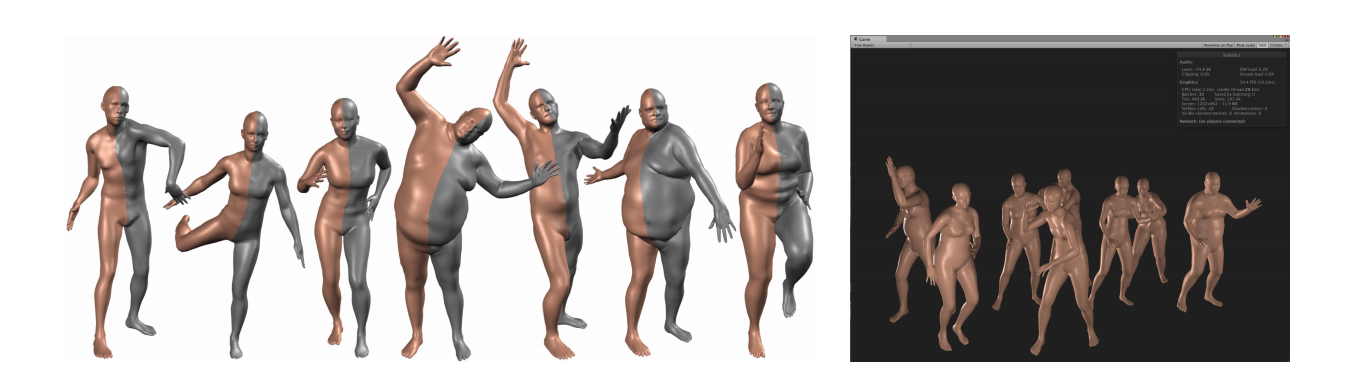
\includegraphics[width=16cm]{figure/smpl}	
	\caption{SMPL is a realistic learned model of human body shape and pose that is compatible with existing rendering engines, allows
animator control, and is available for research purposes. (left) SMPL model (orange) fit to ground truth 3D meshes (gray). (right) Unity 5.0
game engine screenshot showing bodies from the CAESAR dataset animated in real time.}
	\label{smpl}
\end{figure}

SMPL\cite{smpl,smplhomepage}是一个较为成熟的人体建模框架。目标是创造一个可以表示不同形状的身体的,可以随着动作自然的变形的,并且软组织在运动过程中还能发生形变的人体模型。该框架是论文\cite{paper1,paper2}的共同基础,所以为了之后的工作,我们尝试阅读并理解了SMPL的论文和相关代码文件。
\subsubsection{Motivation}
为了解决人体建模时mesh偏移问题,一般商业上的操作手法是手动操作mesh,来修改使用传统模型时出的问题,工作量就比较大。也有人从扫描的人体数据集中学习一个统计的身体模型,但是与商用软件不兼容,没法使用。因此SMPL模型的目标就是,既能使用,又能表示大范围的人体,还要能通过pose来自然的形变,还要有软组织的动力学,做动画的效率高,并且和现有的渲染引擎兼容。

\subsubsection{相关公式和标记}
SMPL将身体形状分解为identity-dependent shape和non-rigid pose dependent shape。这个人体模型包含了$N=6890$个点,与$K=23$个关节。男女的大部分参数都是通用的。模型的输入参数为形状参数$\beta$,和动作参数$\theta$,模型中包含以下几项:
\begin{itemize}
	\item $\bar{\textbf{T}} \in \mathbb{R}^{3N}$:平均的模板形状 (mean template shape),这个时候的pose是zero pose,($\vec{\theta^*}$)
	\item $\mathcal{W}\in \mathbb{R}^{N\times K}$ :各个关节的混合权重
	\item $B_S(\vec{\beta}):\mathbb{R}^{|\vec{\beta}|} \mapsto \mathbb{R}^{3N}$:blend shape函数,将shape参数映射到每一个点上
	\item $J(\vec{\beta}):\mathbb{R}^{|\vec{\beta}|} \mapsto \mathbb{R}^{3K}$:将shape参数映射到每个joint的位置上
	\item $B_P(\vec{\theta}):\mathbb{R}^{|\vec{\theta}|} \mapsto \mathbb{R}^{3N}$ :将pose参数映射到每个点上
\end{itemize}

最终得到的结果就是$M(\vec{\beta},\vec{\theta};\Phi):\mathbb{R}^{|\vec{\theta}|\times |\vec{\beta}|} \mapsto \mathbb{R}^{3N}$ ,将shape和pose参数映射到每个点上。这里的$\Phi$ 指的是学习的模型的参数。

\subsubsection{参数介绍}
作为最重要的参数之一,pose参数是使用axis-angle来定义的,对于每一个joint,都有一个$\vec{\omega}_k\in \mathbb{R}^3$,然后加上原点处的,总共24个关节,就有72个参数。旋转矩阵是使用Rodrigues formula计算得到$W(\bar{\mathbf{T}},\mathbf{J},\vec{\theta},\mathcal{W}):\mathbb{R}^{2N\times 3K\times|\vec{\theta}|\times |\mathcal{W}|} \mapsto \mathbb{R}^{3N}$ ,将rest pose、joint location、pose参数、blend weights权重转化成每个点的坐标量。

关于SMPL的其他参数意义,相关的内容在之前报告中的SMPL源码解析中已经给出,在此不再赘述。

\subsection{Video Based Reconstruction of 3D People Models}

\begin{figure}[H]
    \centering
    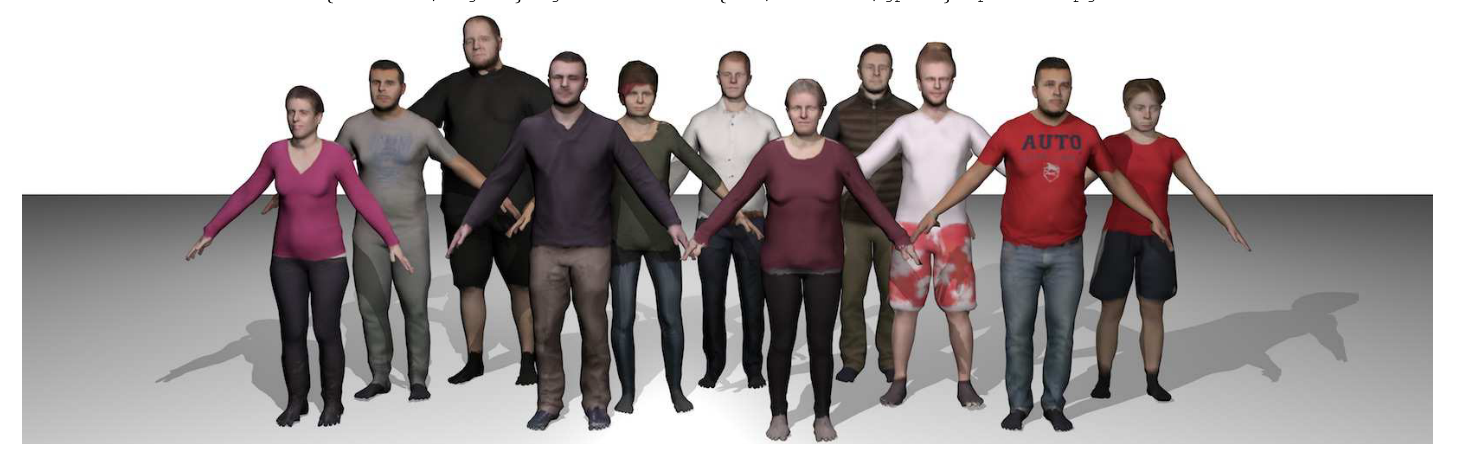
\includegraphics[width=16cm]{figure/paper1.png}
    \caption{Technique in \cite{paper2} allows to extract for the first time accurate 3D human body models, including hair and clothing, from a single video sequence of the person moving in front of the camera such that the person is seen from all sides.}
    \label{paper1_titlefigure}
\end{figure}

\subsubsection{Motivation}
该论文工作的动机是为了对简单的SMPL模型生成结果的不足进行修正,尝试提出一种简单易实现的基于视频图片帧的目标重建框架。对于已有的部分3D重建方法,论文作者将它们的不足概括为:

\begin{itemize}
    \item 使用了高效的扫描设备进行建模数据的采集,价格昂贵而且尺寸巨大,难以被广泛接受和推广;
    \item 使用了多张的静态人物图片进行建,为了得到良好的结果需要目标任务保持静止,对于模特十分困难;
    \item 使用RGBD相机进行数据采集和建模,需要专门的传感器,因此不能直把已有的视频材料作为目标。
    \item 之前的方法都只能对于人物表面的纹理进行方针,难于对内部骨骼姿态进行体现。
\end{itemize}

因此作者将该论文的技术目标定义为:

\begin{quote}
    In this work, we estimate the shape of people in clothing from a single video in which the person moves.
\end{quote}

\subsubsection{Proposed Methods}
针对前述的现有问题和目标,作者在该篇论文中提出了若干个互相补充的优化方法,具体来说,为了实现不同于SMPL的、有衣服纹理和更多细节效果的人体建模,论文提出的方法分为以下几个部分:

\begin{enumerate}
	\item 类似于\cite{2Dkeypoint}中提出的方案,首先使用SMPL生成的模型和2D-level的关键点数据进行拟合,得到3D层面的姿态初始化信息;
	\item 基于得到的结合了3D姿态信息的人体模型,在选择得到的3D point位置,添加基于人体segmentation mask的剪影信息,这个部分添加了一些关键位置的深度信息;
	\item 基于已有的3D-level的点信息,进行逆操作,进行光线投影的计算,从而把不同原始姿态的人体目标统一成相近的姿态(如T-pose),这个步骤被定义为unpose;
	\item 对于得到的标准姿态的3D人体模型,使用SMPL的函数接口,对shape参数和3D点位置进行联合优化,优化的依据来自于unposed rays和3D模型的关键点位置的距离;
	\item 基于视频中的色彩信息和前述步骤得到的无贴图人体模型,进行人物表面贴图的添加。
\end{enumerate}

在原始的SMPL模型中,优化的目标可以概括为:

\begin{align}
		M(\beta, \theta) = W(T(\beta, \theta), J(\beta), \theta, \mathbf{W})\\
		T(\beta, \theta) = \mathbf{T}_\mu + B_s(\beta) + B_p(\theta) 
\end{align}

在原有的优化来源基础上,该论文中提出的方法增加了额外的多项优化能量项,寻求其最小化的过程可以综合表示为一个对一个额外的项目$D$的优化过程,因此上述的优化目标公式变为了:

\begin{equation}
	T(\beta, \theta) = \mathbf{T}_\mu + B_s(\beta) + B_p(\theta) + \mathbf{D}
\end{equation}

在该篇论文的开源代码工程“video-avatar”中,论文的实现被分割成了三个步骤,我们在阅读论文和代码后项目将三个代码部分和论文的方法论相对应,进行相关的知识的梳理总结:(1)姿势重建 (Sec. 3.2);(2)一致形态评估 (Sec. 3.3);(3)帧精炼和纹理图生成 (Sec. 3.4)。该论文的主要贡献在第二步,第一步建立在以前的研究上,第三步中的纹理获取和时变性细节是可选的。

为了评估对象的一致形态(consensus shape),研究者首先计算每个帧的 3D 姿势。他们扩展了 \cite{keepitsmpl}中的方法使其更加鲁棒,并获得更好的时间一致性和轮廓重叠。在第二步,一致形态的计算在Section3.3中有详细介绍。一致形态被高效优化,以最大化地解释每帧实例中的轮廓。由于时间变化导致的衣物变形,这些姿势的一致形态可能和帧轮廓有轻微的错配。因此,为了计算纹理和捕捉时间演化细节,第三步中将用滑动窗口方法对一致形态的偏离进行每一帧的优化(Section3和Section4)。给出精炼的逐帧形态,我们可以计算纹理图。本文的方法依赖于图像的前景分割。因此,研究者使用了\cite{oneshotseg}中基于 CNN 的视频分割方法,并对每个序列用 3-4 个手工分割图像进行训练。为了在单目 3D 人类形态重构中克服模糊性的问题,研究者使用 SMPL 身体模型\cite{smpl}作为起始点。

关于该论文的更多细节,比如三个步骤的具体实现和源代码的解读在之前的报告中已经给出,在每次报告中不再赘述。

\subsection{Detailed human avatars from monocular video}
\begin{figure}[H]
    \centering
    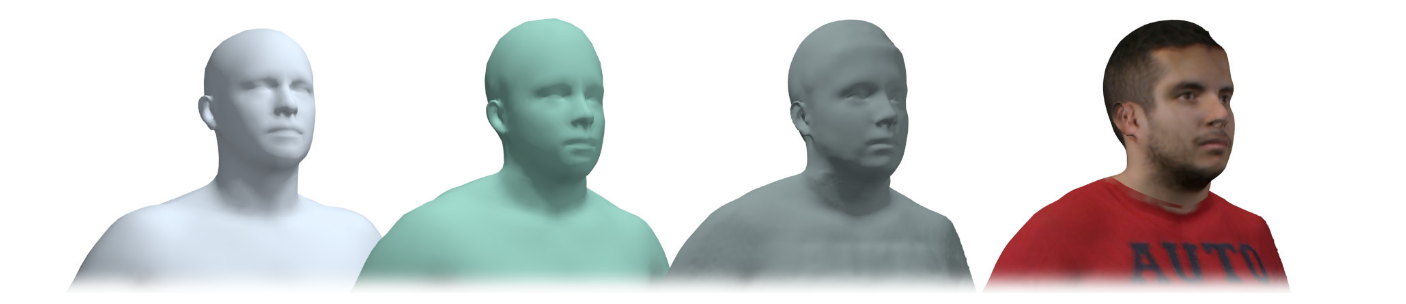
\includegraphics[width=16cm]{figure/paper2.png}
    \caption{Method in \cite{paper2} creates a detailed avatar from a monocular video of a person turning around. Based on the SMPL model, we first compute a medium-level avatar, then add subject-specific details and finally generate a seamless texture.}
    \label{paper2_titlefigure}
\end{figure}

作为本次课程项目的重点,本篇论文基于前述的两篇关键论文的工作进行了改进。本篇论文的核心贡献在于对\cite{paper2}的框架进行优化,加入了更多的先验信息和后验优化的手段,取得了更加细致的人体建模效果。论文中作者把效果优化的来源总结为以下几个方面:
\begin{itemize}
	\item 面部关键点信息的加入,对人面部的细节优化提供了更多的依据;
	\item shape-from-shading技术的加入,增添了更多的空间信息;
	\item 纹理缝合技术,带来了更加细致的表面纹理效果;
	\item 纹理语义处理,消除粗糙的semantic spills的情况,使得人体表面纹理更加真实。
\end{itemize}

为了实现这些方面的优化,论文中提出了若干个具体的操作,包括Subdivision、Medium-level体态重建、表面细节建模和优化后的纹理生成等。
\subsubsection{Subdivided SMPL model}
因为人体建模的实现依赖于三角形或者多边形的mesh,为了实现更加细致的人体表面建模,一种最直接的方法就是使用更多的mesh块来覆盖人体表面,从而允许更加细致的轮廓起伏的描述。论文中使用对mesh边界进行细分(Subdivision)的方法来实现这个目标。
\begin{equation}
	v_{N+e} = 0.5(v_i + v_j) + s_e n_e, (i,j) \in \epsilon_e
\end{equation}

其中$\epsilon$是所以构成一条边的顶点对,$n_e$是所有点对的平均模量。通过这种方法,原本拥有$N=6890$个顶点的SMPL模型被细分称为拥有$N^\prime = 110210$的更加细致的人体建模模型。
\subsubsection{Medium-level体态重建}
为了更好的建模头发、衣服等中等层面的细节,论文提出了一种中层体态重建的方法。尽管类似的工作已经被许多之前的工作所提出,本文提出的方法仍然有很多新颖的地方,包括针对面部的特别优化,以及优化过程的设计等。具体的来说,优化过程中,如同\cite{paper1}一样,人体姿态被统一为标准的姿态,但是通过额外添加面部表面点的坐标数据,模型得以展现更多的面部细节。另一方面,这个步骤中同时优化了模型的细节深度信息、面部细节和一个正则惩罚项,从而在保证了面部信息的优化的同时不会显著劣化已有的细节信息。为了方便,对于面部坐标点的获取可以直接通过OpenPose\cite{openpose}实现。

另一方面,在进行细节优化的时候,优化的具体操作也被特别设计。使用barycentric插值,每个面部的坐标点,都被映射到了一个临近的已有mesh顶点(考虑到面部坐标点庞大的数量,如果在没有进行前述的subdivision的原始模型上,稀疏的mesh顶点会导致这种映射非常不可靠)。通过计算这个被选中的顶点和面部坐标点之间的距离,以及它和重建相机给出的光线路径之间的距离,在一个unpose\cite{paper1}之后的目标姿态空间内,优化的最终距离表示为:

\begin{equation}
	\sigma(l, r) = l \times r_n - r_m
\end{equation}

其中,$r=(r_m, r_n)$是对原坐标空间映射到Plucker坐标系之后的结果。由此,最终优化过程中的面部能量项表示为该距离项在Geman-McClure损失函数$\rho$处理之后的加权合并:

\begin{equation}
	E_{face} = \sum_{l.r\in \mathcal{L}} w_l\rho(\sigma(l_l, r_r))
\end{equation}

\subsubsection{表面细节建模}
论文另一个关键的部分是对于表面细节的优化,这个步骤较为复杂,也是本篇论文中最特别的创新。这个部分的实现可以分为两个步骤:\\

\chapter{Step 1.参考法向量的生成}\\
因为视频是通过2D视觉进行展示的,是简单的RGB信号,并没有深度信息,所以想通过2D视觉信息生成3D空间内的表面法向量需要进行低维度的信息提炼呵推测。本文实现这一步骤的方法是可以使用可以很好利用阴影等对比信息的shape-from-shading\cite{shapefromshading}方案。具体来说,当在原始的人体模型上仅仅添加shape-from-shading的信息时,我们可以认为此时模型表面的mesh法向量是比较可信的,因为shape-from-shading方法中利用阴影信息对于空间结构的推测已经被证明是相对比较可信的。该步骤生成的法向量会在之后的步骤中作为参考法向量参与到模型的优化之中。

\chapter{Step 2.表面细节优化}\\
对表面细节的优化目标由多个优化项目共同组成,可以表示为:

\begin{equation}
	argmin_{\mathbf{D},s} \sum_{j\in C} (\lambda _jE_{silh,j} + \lambda _j w_{face}E_{face,j}) + w_{sfs}E_{sfs} + E_{regf}
\end{equation}
其中$E_{silh}$和$E_{face}$已经在\cite{paper1}和上一小节被分别介绍过。该公式引入的最重要的优化项目为$E_{sfs}$,它是基于shape-from-shading结果的,对于表面细节的项目关键。具体来说,在优化过程中,模型表面的mesh方向会不断发生变化,考虑到这个综合的优化过程引入了包括面部标记、基于图像分割的轮廓信息等太多额外的信息,这些信息在尝试提供额外的细节信息的同时也可能会对耦合区域的mesh方位发生影响,而且这种影响往往是负面的,因为mesh作为唯一的可变化的表面表现单元,会主动被调节去适应提供的先验信息,所以为了更加准确的表面信息,$E_{sfs}$致力于对mesh方位偏移的修正。这个修正的基准便是之前在单独添加shape-from-shading信息时候生成的参考法向量。所以,论文定义:

\begin{equation}
	E_{sfs} = \sum^{k+m}_{f=k-m}\sum_{i \in V} || n_i - \tilde{n_i}^{f} || ^2
\end{equation}

而$E_{regf}$作为一个正则惩罚项,分别对四个项目进行惩罚:

\begin{itemize}
	\item 相邻帧中对应mesh的方位差异;
	\item 表面mesh的光滑程度(基于Laplacian Smoothness优化);
	\item 同论文\cite{paper1}一样,对于形态一致性决策的优化;
	\item 对于组成mesh的若干边长度差异的惩罚;
\end{itemize}

\subsubsection{优化的纹理生成}
在对表面纹理的处理上,本文分为了各部分纹理生成、纹理语义先验信息处理和最后的纹理合并三个步骤。
\subsubsection{复现难点总结}
坦白来说,作为一个课程作业,在有限的时间内复现本文是非常困难的,特别还是在我们小组组员都对3D模型重建的相关知识之前并没有了解的前提下。我们在阅读论文的过程中也遇到了许多困难,在之后尝试和论文的作者Dr. Weipeng Xu进行了联系,在一段时间的沟通和梳理之后,我们认为完整复现本文存在以下若干的难点:

\begin{itemize}
	\item 论文中使用的shape-from-shading方法来自于文献[84],该文献的作业也为马普所人员,他们内部拥有原始代码。但因为[84]的代码并没有公开,所以我们并不能直接使用,而对其进行复现的难度也较大;
	\item 对于Section 3.2中使用的[14]的方法,该模型必须在目标数据集的训练集部份上进行fine-tune,否则很难得到可用的结果,具体的方法是手动标注一个base frame的ground truth,之后迭代进行训练,考虑到相机标定和数据准备等过程,该部分任务会比较繁重和困难;
	\item 纹理生成的部分中,论文提供的细节信息很少,我们很难从其中提取出来完整的实现流程,同时也存在大量的主观参数设定的问题,可能需要多次的尝试,带来诸多的困难。
\end{itemize}

\section{部署使用Video-Avatar代码}
基于\cite{paper1code}中的代码实现,我们迈出了项目创新部分工作的第一步。因为关于论文\cite{paper1}的源代码(Video-Avatar)已经被作者开源\cite{paper1code},我们直接获取了这个开源的工程,尝试进行部署和使用。

\subsection{项目部署}
\subsubsection{获取SMPL工程}
为了实现目标工程,首先需要下载SMPL的项目代码\cite{smplhomepage}。为了方便,我们推荐使用Python API的版本。另一方面,我们还需要下载一个依赖库SMPLify\cite{smplifyhomepage},相关的注册等流程不在此赘述。

\subsubsection{获取数据集}
和Video-avatar代码一同发布的还有一个用于进行3D人体重建的数据集people-snapshot\cite{paper1homepage}。这个数据集中包含了经过处理的以近景人物作为主题的视频文件、视频中人物的mask和keypoint标注文件,以及在之后会用到的相机标定文件等。

\subsubsection{部署项目依赖}
我们直接从github\cite{paper1code}获取项目代码并进行必要的部署工作,部署默认在linux环境下进行。相关的编译依赖为Ubuntu 16.04 LTS默认版本和Python2.x。

\begin{lstlisting} 
# 获取源代码文件
git clone https://github.com/thmoa/videoavatars.git videoavatars
cd videoavatars/vendor
mkdir smpl
cd smpl

# 对smpl工程文件进行链接
ln -s <path_to_smpl>/smpl_webuser/ ./smpl_webuser
ln -s <path_to_smpl>/models ./models
cd ..

# 对smplify工程文件进行链接
mkdir smplify
cd smplify
touch __init__.py
ln -s <path_to_smplify>/code/models ./models
cp <path_to_smplify>/code/lib/*.py ./

# 修改vendor/smplify/sphere_collisions.py中的line14为:
# from vendor.smpl.lbs import verts_core
\end{lstlisting}

\subsection{工程运行}
在完成代码部署之后,可以尝试使用代码文件,在作者的代码仓库中简单说明了不同的代码文件的作用:

\begin{lstlisting} 
The software consists of three parts:
1. step1_pose.py: pose reconstruction
2. step2_consensus.py: consensus shape optimization
3. step3_texture.py: texture calculation

Starting the scripts will display usage information and options.
Additionally, we provide helper bash scripts for easier processing of 
our dataset.

The scripts in prepare_data might help you to process your own data.
\end{lstlisting}

同时,因为依赖库等原因,在正式运行代码之前,我们可能还需要一些辅助的工作,具体的过程:

\begin{lstlisting} 
# 安装依赖库
conda/pip install opencv-python
conda/pip install h5py
pip install chumpy
pip install opendr
pip install tqdm
sudo apt-get install python-tk

# 对程序需要的环境进行准备
cd <path_to_videoavatar>
cp -r <path_to_dataset>/case
mkdir output1
mkdir output2

# 开始运行程序代码,"case"为选择的数据集对象
./run_step1.sh case output1
./run_step2.sh case output2
\end{lstlisting}

\subsection{生成模型的渲染和可视化}
使用前述的videoavatar工程文件生成了目标人物的建模结果之后,为了直观展示效果,还需要对结果文件进行渲染和可视化,这个部分我们利用了一些已有工具,并且自己编写了更加方便的脚本进行操作。本节简述小组在这方面的相关工作。

\subsection{对obj模型文件的优化}
videoavatar工程生成得到的最终obj模型文件在进行最终的可视化之前,还需要进行一些优化处理。主要包括对于法向量的添加、uv映射和贴图的优化以及对mesh的细化等。
\subsubsection{添加法向量}
为了加入反射来展现出模型的真实感,需要计算模型表面mesh的法向量进而获得光照情况。论文代码生成的 .obj 文件中并没有加入法向量。为了得到法向量,使用OpenGL中导入模型时计算法向量。
\subsubsection{uv映射和贴图}
代码生成的贴图是和模型的uv映射的契合的,只要贴上贴图即可。由于代码 .obj 已经定义了uv映射,因此只要指定贴图文件即可。
\begin{figure}[H]
	\centering
	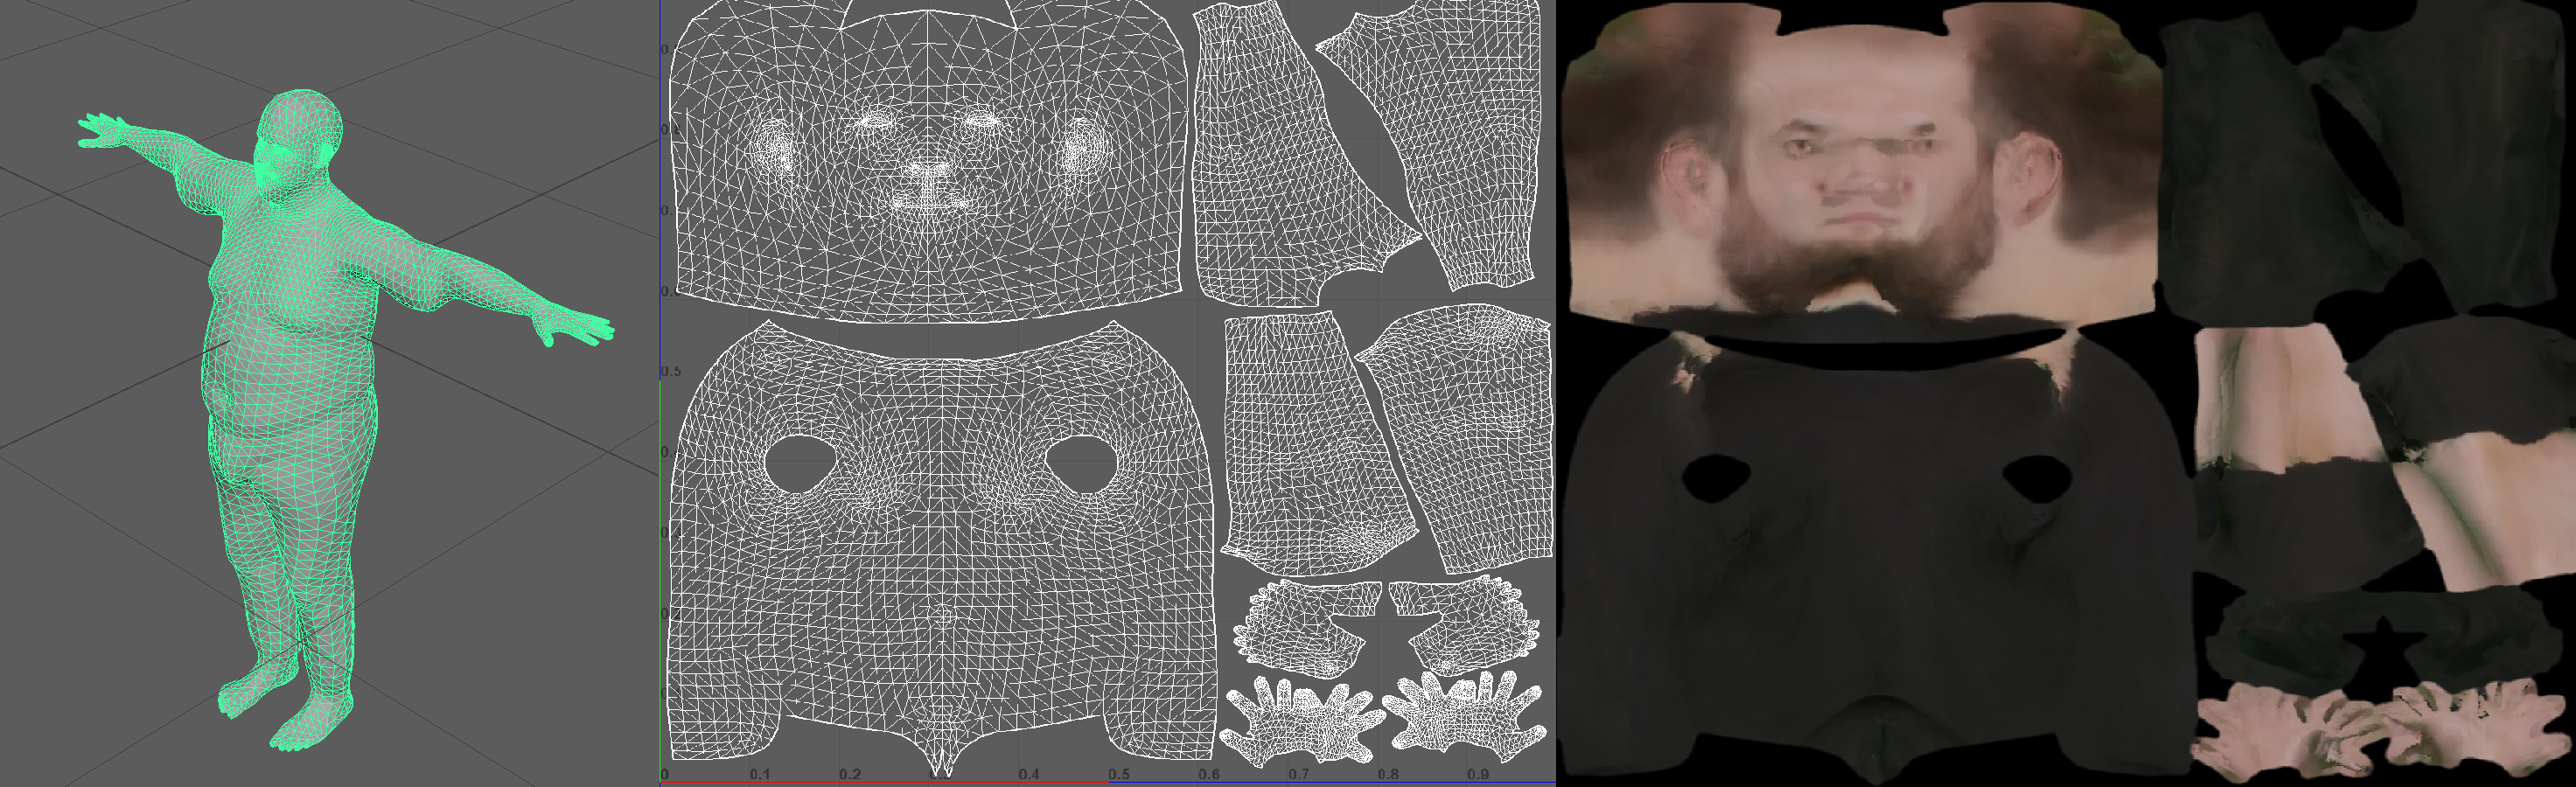
\includegraphics[width=16cm]{figure/uv}
	\caption{渲染时需要使用的贴图文件示例}
\end{figure}

\subsubsection{细化mesh}
对于已有的mesh分布,我们使用assimp库在导入模型时会将过大的mesh细化为小网格,并且所有mesh均用三角形表示。同时,由于实时渲染的资源限制,在单次Draw()中能绘制的的三角形数目和最大顶点缓冲是有限的。
通过指定mesh的网格限制和顶点限制可以有效的缓解这个问题。

\begin{lstlisting} 
Assimp::Importer importer;
// aiProcess_SplitLargeMeshes: 将大Mesh分割成小的子Mesh
const aiScene* scene = importer.ReadFile(modelFile \\
			, aiProcess_SplitLargeMeshes);

// Vertice最多个数
#define AI_SLM_DEFAULT_MAX_VERTICES 10000000
// Triangle最多个数
#define AI_SLM_DEFAULT_MAX_TRIANGLES 10000000   
\end{lstlisting}

经过前述的步骤,我们最终可以得到具有完整效果的videoavatar实现,我们对\cite{paper1homepage}数据库中的部分视频进行了测试,得到了一些取样效果如Fig.\ref{videoavatarsample}所示。

\begin{figure}[H]
	\centering
	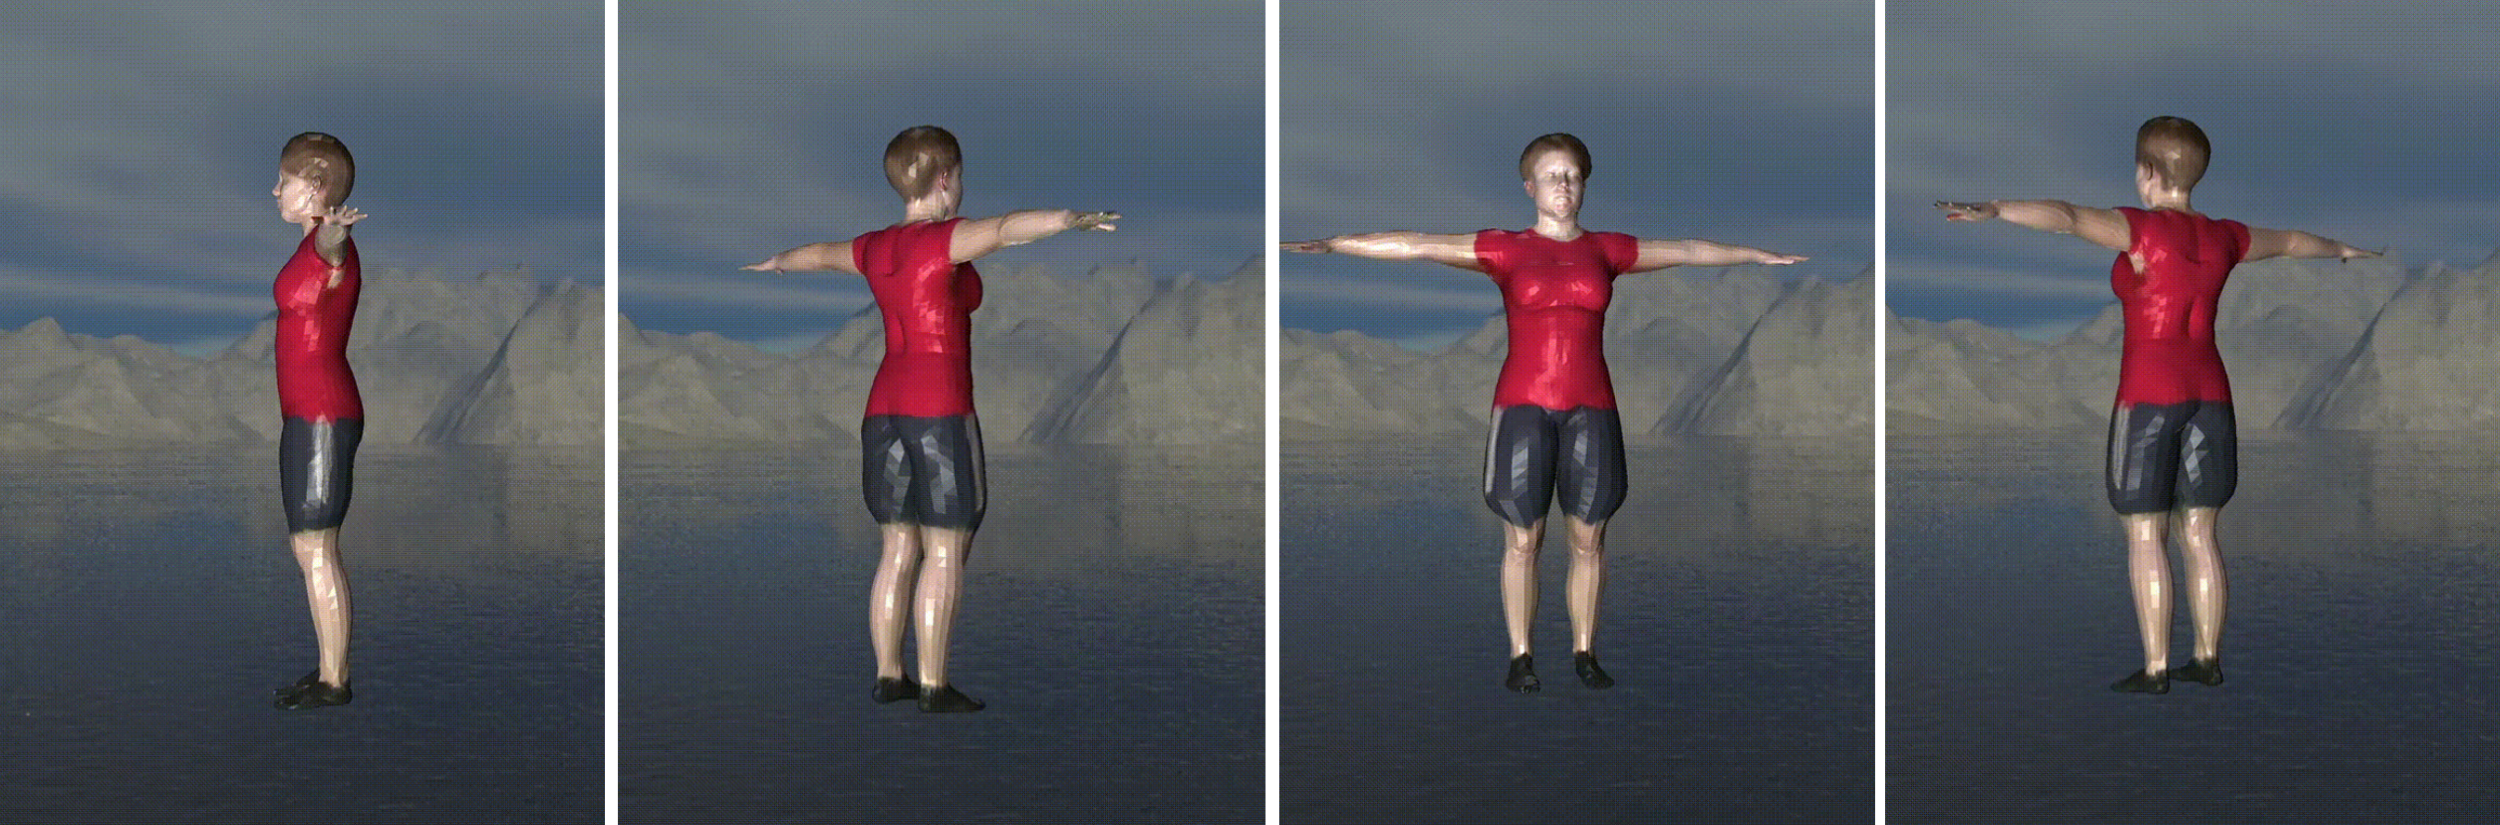
\includegraphics[width=16cm]{figure/videoavatar_4angle}
	\caption{取样于people-snapshot数据集的videoavatar多角度效果示意图。}
	\label{videoavatarsample}
\end{figure}

\subsection{自制渲染工具}
为了更加简便地对得到的obj文件和贴图进行合并渲染,我们还基于windows的批处理机制自行制作了一个针对该项任务的只需要简单操作便可以完成操作的渲染工具,相关的细节在Appendix C中给出。


\section{优化3D重建项目}
\subsection{基于Video-avatar已有代码的参数优化}
在videoavatar的工程文件中,包含大量需要主观设置的参数,对这些参数进行调整可能会带来模型生成能力的优化。具体的来说,我们主要调整了公式Eq.\ref{adjust_term}中不同项目之间的权值。

\begin{equation}
	E_{cons} = E_{data} + w_{lp}E_{lp} + w_{var}E_{var} + w_{sym}E_{sym}
	\label{adjust_term}
\end{equation}

优化后的效果如Fig.\ref{adjust_compare}所示,可以看到,因为视频中的同学是偏瘦的体型,在videoavatar的默认参数下,试图往其身高对应的多数体型进行优化,得到的建模结果(右)较真人更加胖一些,在进行参数调整之后,得到的建模结果(左)和真人体型更加相近了。

\begin{figure}[H]
	\centering
	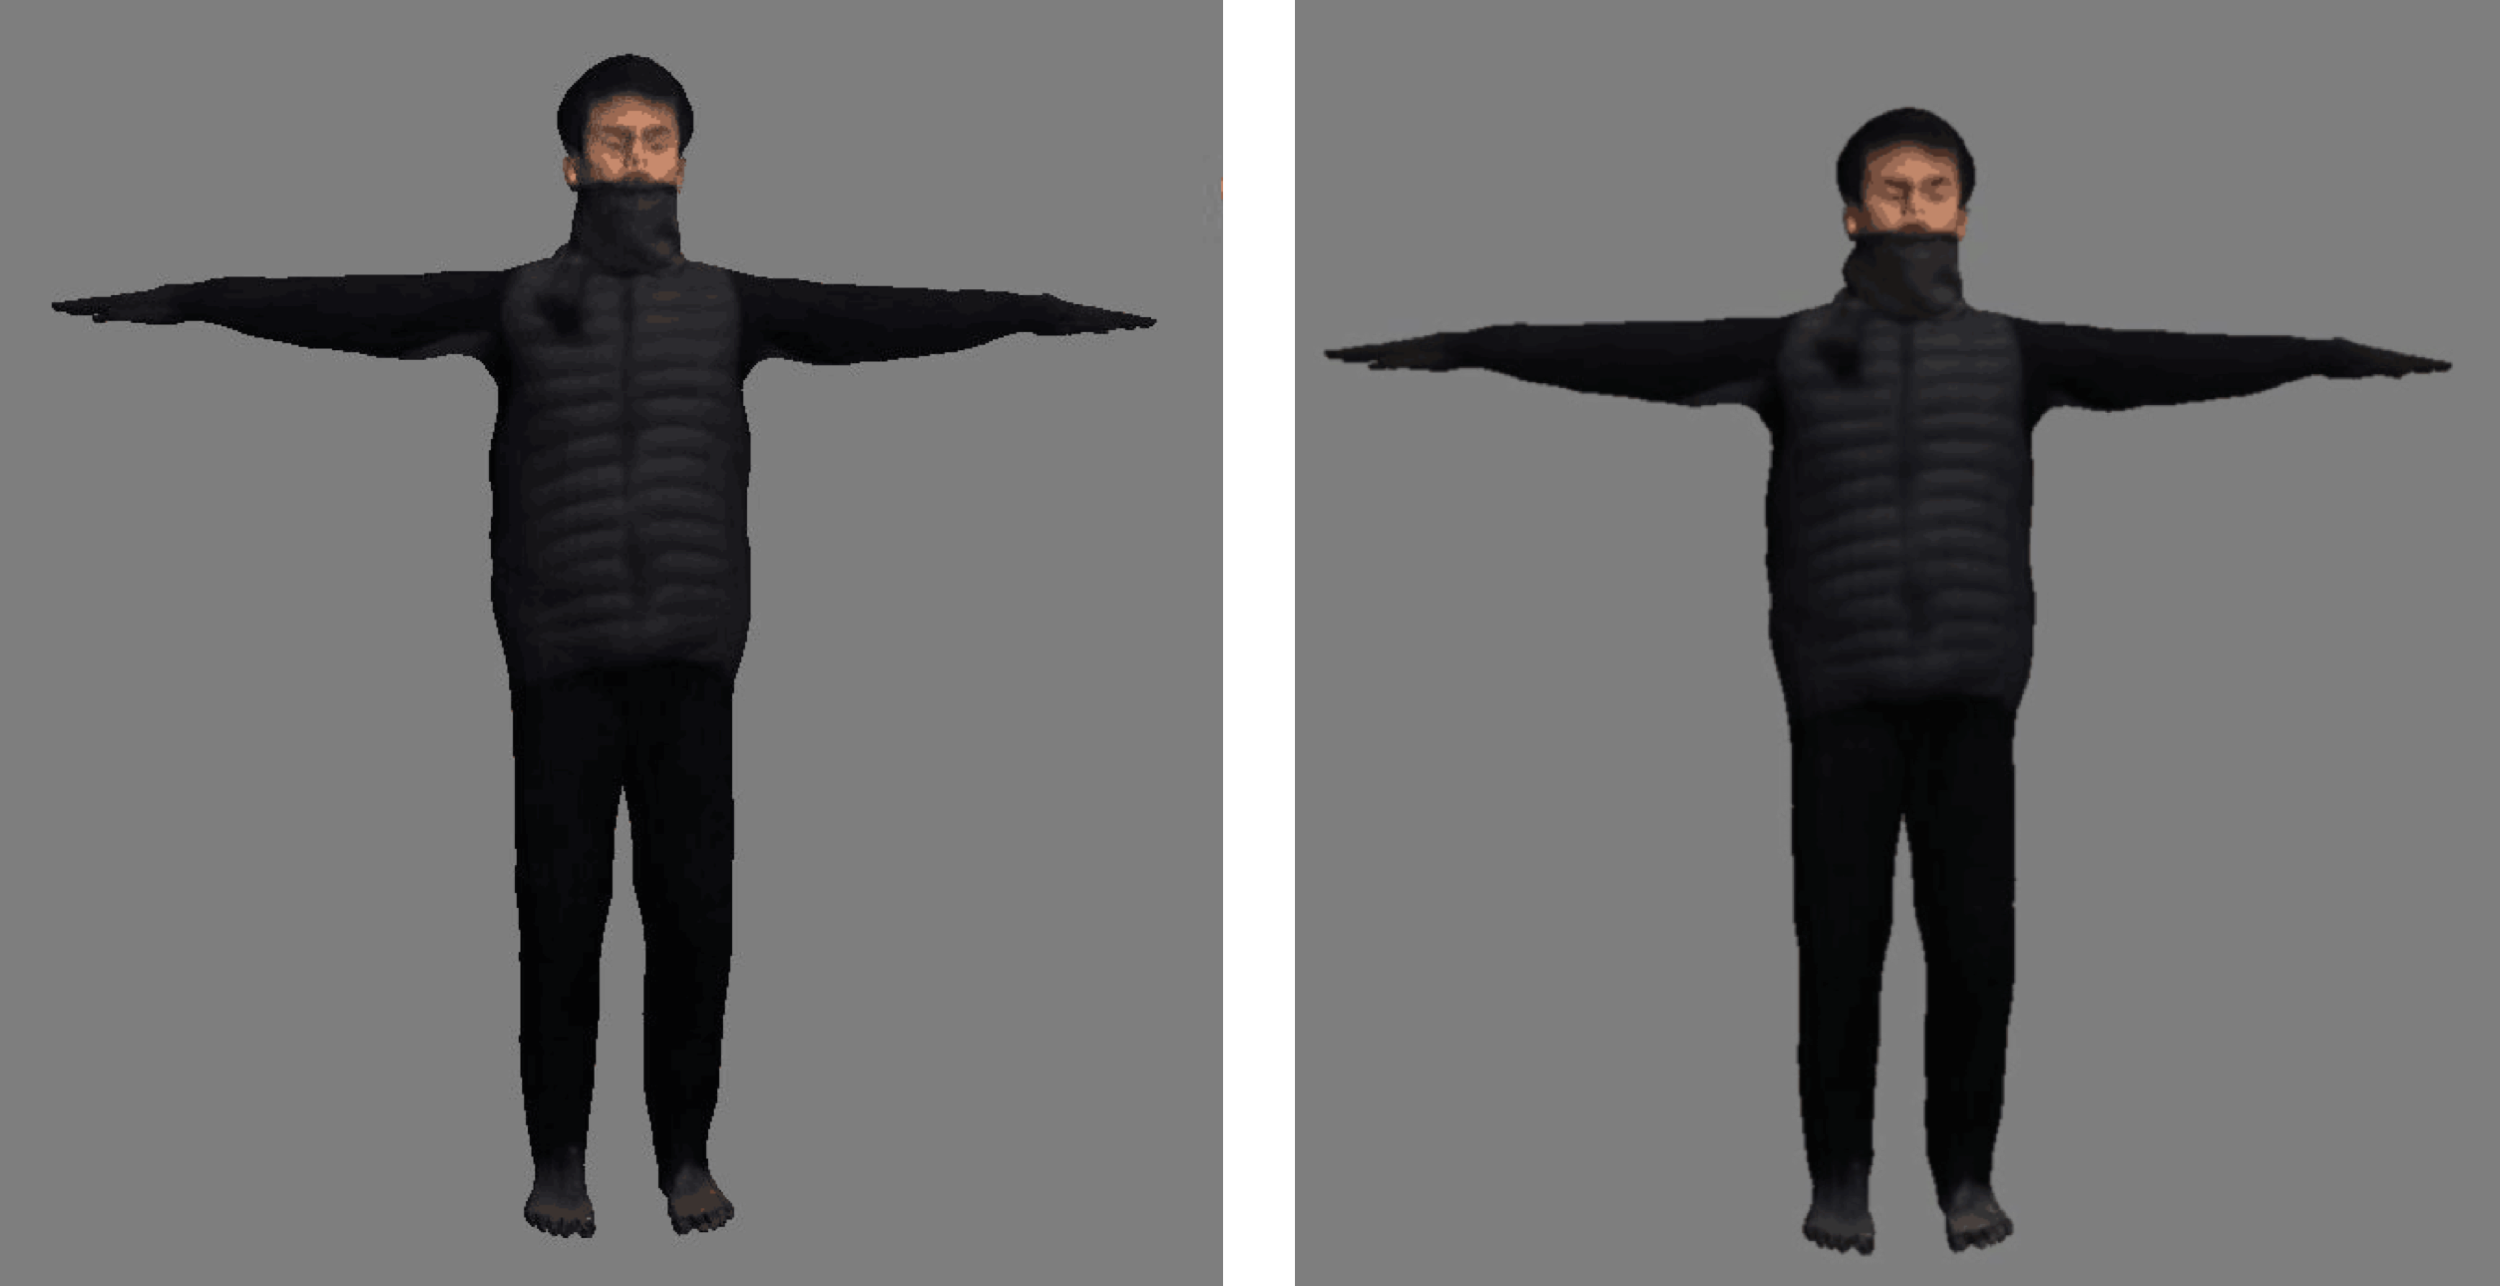
\includegraphics[width=14cm]{figure/adjust_compare.png}
	\caption{在对videoavatar代码进行参数调整的前后对同一帧视频中的人体得到的不同建模结果,左图为参数调整之后的建模结果,右图为使用默认参数时的输出结果}
	\label{adjust_compare}
\end{figure}
\subsection{Detailed human avatars实现}
\subsubsection{Facial Landmarks}
针对\cite{paper2}中提到的利用facial landmarks等信息进行面部建模细节优化的方案,我们小组也进行了复现。这个部分的步骤较为繁琐,细节可见\cite{faceoptimization}。

该部分的关键是利用额外添加的面部关键坐标点(landmarks)对对应区域的顶点(vertex)位置进行小幅度的调整,从而使其更加接近于建模模特的本来面部特征。

\chapter{生成需要的face landmarks文件}
我们使用Openpose\cite{openpose}框架识别得到了目标人物面部的landmarks数据,该数据格式和对应的面部位置可见Fig. \ref{openposeface}。

\begin{figure}
	\centering
	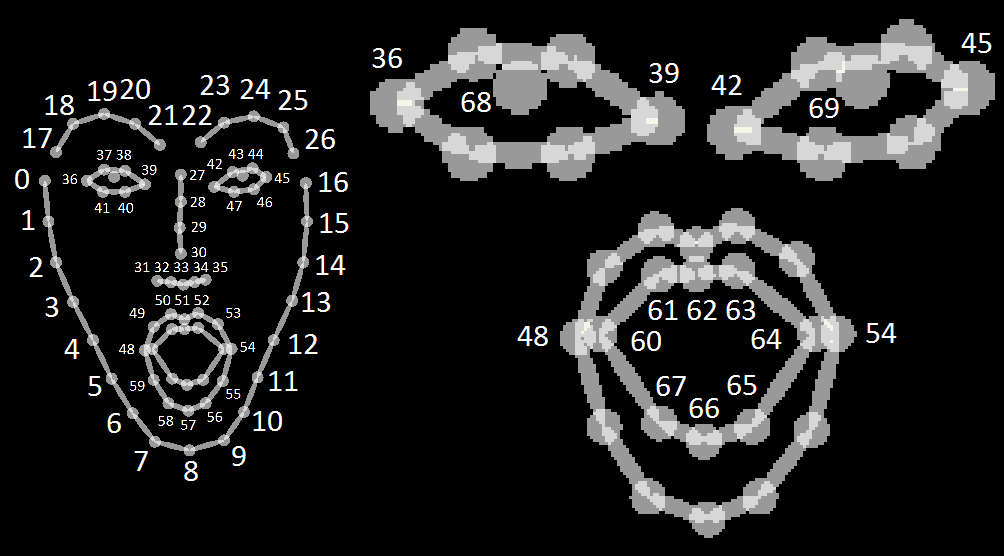
\includegraphics[width=14cm]{figure/openpose_face}	
	\caption{Openpose Face Keypoint Detector输出的人体面部关键点位置分布。}
	\label{openposeface}
\end{figure}

使用face2hdf5.py文件, 根据OpenPose识别出的face keypoint文件生成face\_landmark.hdf5:

\begin{lstlisting}
$ python face2hdf5.py <path_to_subject_directory> <face_landmark.hdf5>
\end{lstlisting}

\chapter{源代码修改工作}
为了实现对面部细节的优化,在viedeoavatar代码文件的基础上,我们进行了大量的改动。

\begin{itemize}
	\item face2hdf5.py: 读取由OpenPose处理得到的每帧画面的face landmark识别结果,将多个json文件中的相关数据将存储为一个dataset,并保存为hdf5格式。实现过程类似于/prepare\_data\\/2djoints2hdf5.py;
	\item bodypart.py:定义了函数获取SMPL模型中面部的vertex id;
	\item frame.py:定义了函数setup\_frame\_rays\_paper2,用于替换原有的setup\_frame\_rays,新函数比原来多了面部landmark数据,并且为每一个frame对象新增了face\_landmark和face\_rays两个属性;
	\item rays.py:定义函数,从2D landmark构造camera rays,从而在之后的优化过程中获取优化损失项;添加函数对3D vertex和landmark rays进行匹配,并对rays进行unpose处理,整个过程类似于 select\_and\_unpose函数;添加了ray\_face函数,计算E\_face能量项;
	\item step2\_consencus.py:在fit的过程中加入了face\_consensus的项目等,利用来自于面部关键点的信息进行细节优化;
\end{itemize}

详细的代码实现可见Appendix D部分。总的来说,在这个部分中,我们的工作仍然在videoavatar已有的框架下进行,同样复用了SMPL工程中的优化接口等内容,极大地减少了工程负担,但是仍旧花费了我们大量的时间。更为重要的是,因为openpose对于面部细节估计并不是高度可信的,我们很难将E\_face的项目比重设置过大,而且在实现过程中需要对大量的主观参数进行设定。在保证模型大体准确的前提下,我们进行了大量的尝试,产生了类似于Fig.\ref{face_compare}的效果比对,但是可以发现的是,对于面部细节的优化带来的直观效果改变并不明显,我们小组认为想要更加突出地体现该部分的作用,需要更加准确的Facial landmarks数据和更为合理的参数设置。


\begin{figure}
	\centering
	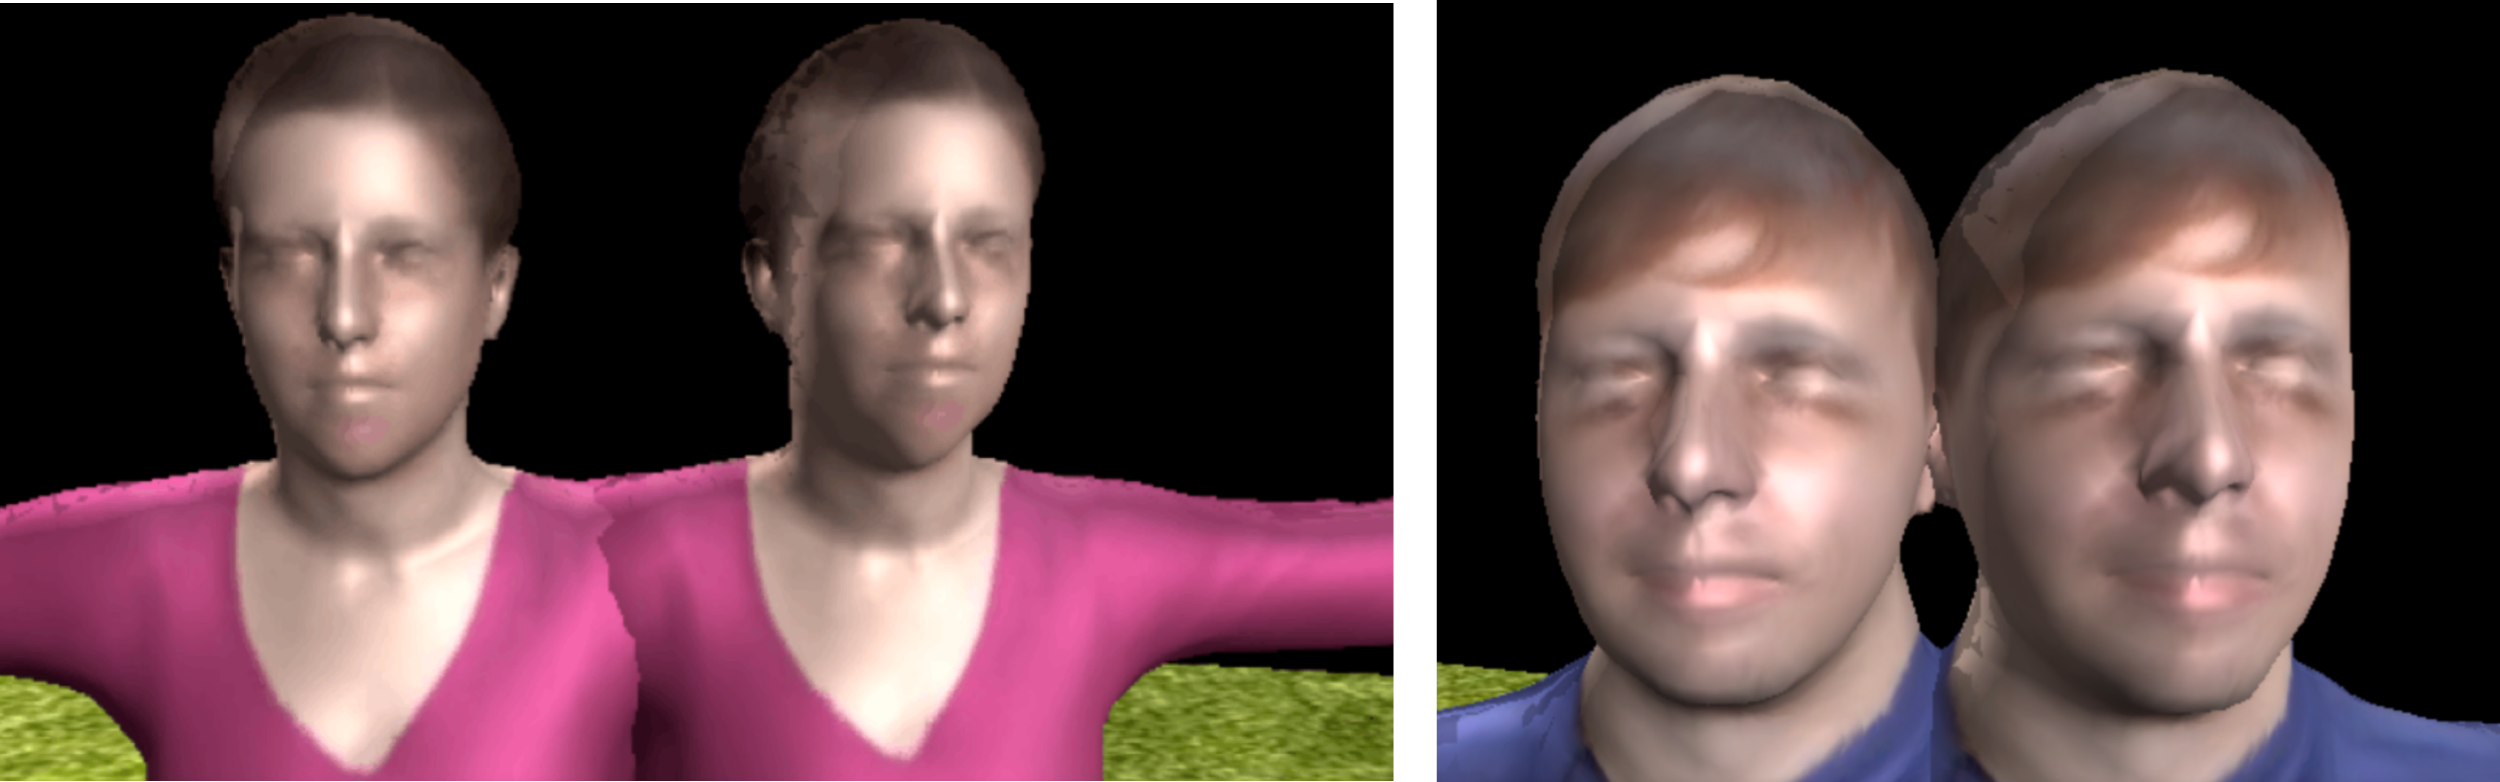
\includegraphics[width=16cm]{figure/faceoptimization.png}
	\caption{加入facial landmarks信息后优化结果对比图,每张图片的左侧模型为优化之后的,右侧为原始模型效果图。}
	\label{face_compare}
\end{figure}

\subsubsection{Subdivided SMPL body model}

原本的smpl的模型中,使用了6890个点,13776个面。对于一个3D的model来说,这样的点面数量略有稀疏,在模型展示的时候可以明显的分辨出表面的mesh快,所以作者在论文的第一部分中就将模型做了细化,细化后的模型将拥有110210 点,和220416个面。细化后的模型更加细致平滑,人体表面没有明显mesh。

由于我们的电脑的内存的资源有限,而模型的大小和顶点的平方成正比。如果按照论文中的要求,顶点的数量增加了16倍,导致所需要的内存资源增加了256倍,会导致memory error所以我们做了一定的简化,最终生成的模型的顶点数量是之前的4倍,总共27554个顶点。

\chapter{Part 1: 应用的依赖库}

\begin{lstlisting}[language=python]
# 读取模型pkl
import cPickle as pkl
import scipy.sparse as sp
# 非线性规划模块,特别的,我们这里使用scipy模块中
# 的optimize进行优化,使拉普拉斯惩罚项的值最小。
from scipy.optimize import minimize
# 可视化展示的模块
from OpenGL.GL import *
from OpenGL.GLU import *
from OpenGL.GLUT import *
# 进行矩阵的运算
from numpy import *
import numpy as np
import sys	
\end{lstlisting}


\chapter{Part 2: 建立smpl模型图矩阵}\\
由于我们知道了每个face是由哪些顶点组成的,即哪些顶点是相邻的,所以我们可以由此建立起该模型的图相邻矩阵。每一个新加的顶点的初始位置是每条边的中值,这部分的代码较为繁杂,详见Appendix B。

\chapter{Part 3: 对图矩阵进行归一化}
\begin{lstlisting}[language=python]
weight = adj.sum(axis = 1)
jj = 0
for x in adj:
    if weight[jj]>0:
        adj[jj] = x / weight[jj]
    jj= jj+1    
kk = 0	
\end{lstlisting}


\chapter{Part 4: 对mesh光滑性进行拉普拉斯优化}
将所有的邻接点乘上对应的矩阵减去该点原有的位置,可以得到拉普拉斯坐标下各个点的位置,我们可以通过多轮优化得到其最小值。
\begin{lstlisting}[language=python]
def opt(node_position):
    global adj,kk,new_dd,node_num
    kk = kk+1
    node_position = np.reshape(node_position,(node_num-6890,3))
    res = adj.dot(np.concatenate([v_template,node_position]))- \\
    	np.concatenate([v_template,node_position])
    res = (res*res).sum(axis = 1)
    res = pow(res,0.5).sum()
    if kk %500 == 0:#itelate 500 and stop
        kk  = 1
        print res
        new_dd = node_position #only new node
        new_dd = np.concatenate([np.reshape(node_position,(node_num-6890,3)),	\\
        	v_template]) #new node and fix node
        #new_dd = v_template #fix node
        main() #show 3D model
        y=input("to stop the procedure") #stop
    return res	

# 使用minimize自带的SLSQP进行非线性规划。
result = minimize(opt, new_node_position, method='SLSQP')
\end{lstlisting}

经过前述的工作,我们在原始的SMPL点阵规格的基础上进行了细化,得到了更加密集也更加细致的人体表面坐标点建模,相关的效果图见Fig.\ref{subdivision}.

\begin{figure}[H]
	\centering
	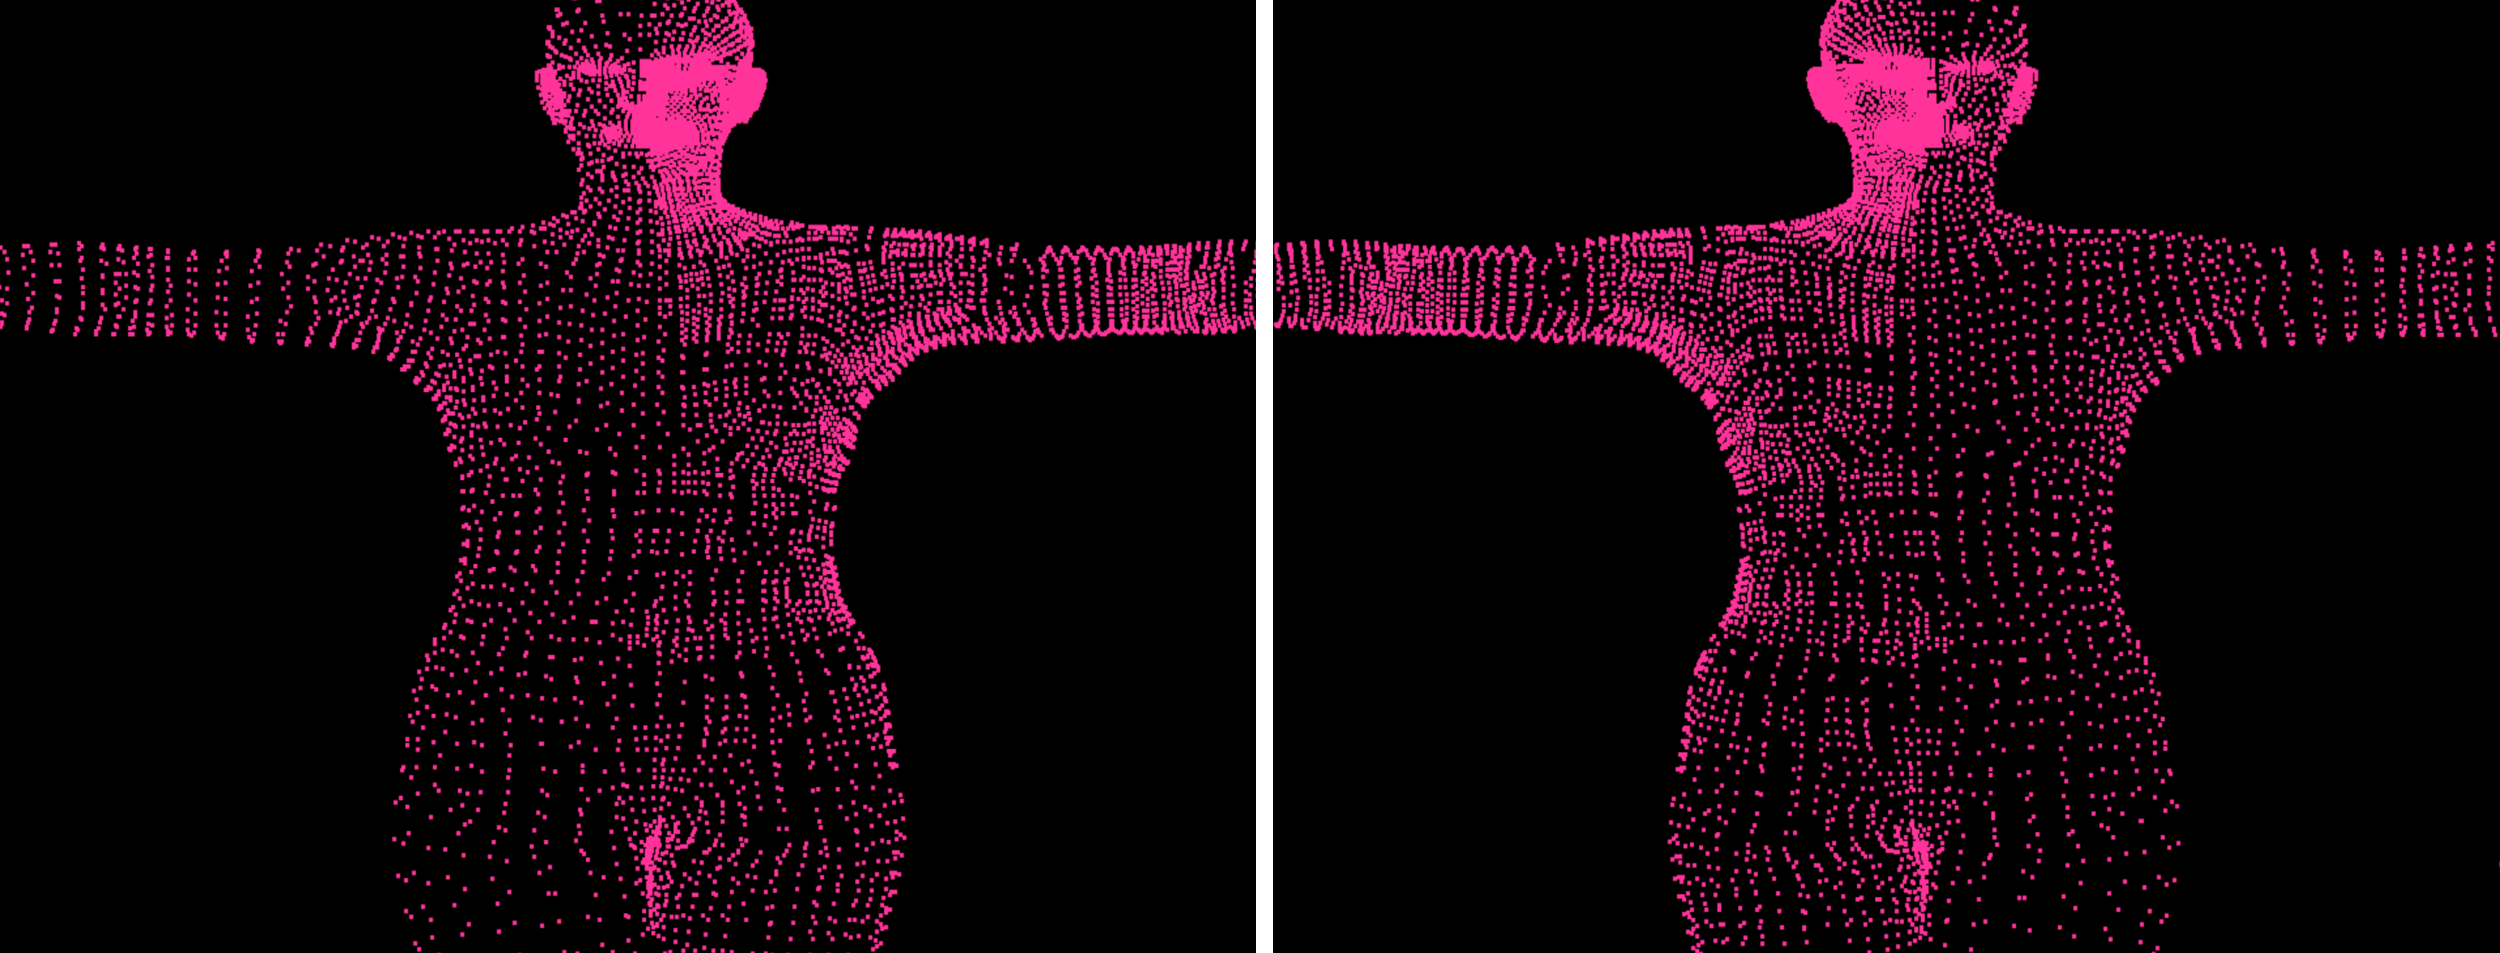
\includegraphics[width=16cm]{figure/subdivision}
	\caption{在进行表面点阵细化(Subdivision)工作前后的效果示意图,为了更加直观的表现工作的效果,我们仅对人体身体的半侧进行了点阵的细化。}
	\label{subdivision}
\end{figure}

\section{自拍视频进行建模实验}
为了更好的验证我们的代码部署和修改工作,小组成员还自行拍摄了视频,尝试进行基于自建数据的人体建模。

\subsection{准备工作}
在得到基本的视频之后,对其需要进行一些前置处理工作,具体来说包括mask生成、关键点标注和相机标定等。具体的来说,需要得到以下的准备文件:

\begin{lstlisting}
camera.pkl 			# 相机标定文件
face_landmark.hdf5		# 面部关键点文件
keypoints.hdf5			# 躯体关键点文件
masks.hdf5			# 语义分割文件
\end{lstlisting}

\subsubsection{相机标定数据获取}
为了进行自拍视频的建模,camera.pkl中需要记录一些关键的相机参数,因为在拍摄过程中,我们尽量保证了人体中部和画面中部的对齐,所以相机数据的中心点位置我们使用默认值即可。长度和宽度设定为1080*1080像素。对于“像素焦距”的计算颇为复杂,因为一般的拍摄设备只提供成像时的毫米焦距数据,“像素焦距”的数值需要利用下面的方法进行计算得到:

\begin{align}
	fx = u \times dx \\
	fy = v \times dy 
\end{align}

其中$u$和$v$分别时相机内参数矩阵的设定值,一般可以直接设定为1,另外还有:
\begin{align}
	dx = (24.5 \times \frac{1}{ccd\_size} \times \frac{image\_X}{image\_Y})/image\_X \\
	dx = (24.5 \times \frac{1}{ccd\_size} \times \frac{image\_X}{image\_Y})/image\_Y
\end{align}
	
其中$ccd\_size$是相机的硬件参数,即传感器的CCD尺寸,一般以英寸为单位,24.5是为了将长度量纲统一到毫米,$image\_X$和$image\_Y$是图片长宽方向的像素数,在我们处理后的自拍视频中,数值均为1080。

\subsubsection{Mask标注或生成}
在制作模型的时候我们需要得到人物的mask和smpl模型的2d投影进行匹配。如何在图片中准确的找出人物的mask是该优化的关键。我们可以使用开源的deep mask框架,也可以通过CNN进行训练。我们在尝试了deepmask\cite{deepmask}之后发现识别的精度并不好,对我们模型的优化有极大的影响。之后尝试了通过手动标注mask的方式(选择了LabelMe\cite{labelme}工具进行标注),但是效果仍然不佳,所以使用了图像处理(边缘检测,二值处理,滤波,开闭操作)生成了较为精确地mask:

\begin{figure}[H]
	\centering
	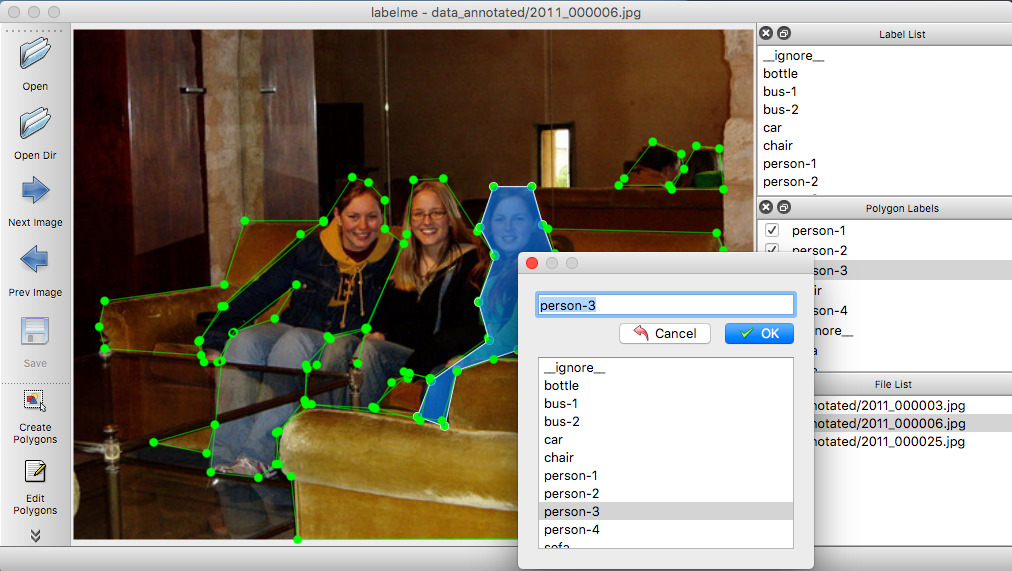
\includegraphics[width=14cm]{figure/labelme}
	\caption{labelme工具使用示意图}
\end{figure}

\begin{enumerate}

\item 因为我们得到的图像是一个RGB的彩色图像,为了方便我们的处理,先将图像进行灰度处理。这里采用了加权平均法,对三个通道进行灰度的转换:

\begin{lstlisting}[language=python]
img = cv.CreateImage(cv.GetSize(image), image.depth, 1)
for i in range(image.height):
    for j in range(image.width):
        img[i,j] = 0.3*image[i,j][0] + 0.59*image[i,j][1] + \\
        	 0.11*image[i,j][2]
\end{lstlisting}

\item 对结果进行中值滤波,过滤噪声点,使最后生成的mask更加准确,并且使用计算机形态学中的开操作填补上mask中的一些小洞,使的mask看上更加的准确。这里我们采用10*10的卷积核:

\begin{lstlisting}[language=python]
# 中值滤波过滤噪声
img = cv2.medianBlur(img,5)

# 使用开操作修补mask剪影
kernel = cv2.getStructuringElement(cv2.MORPH_RECT, (10, 10))
th1 = cv2.morphologyEx(th1, cv2.MORPH_OPEN, kernel, iterations=5)
\end{lstlisting}

\item  对图像进行边缘的检测,得到大致的轮廓。我们使用的'Adaptive Mean Thresholding', 'Adaptive Gaussian Thresholding'这两种边缘检测的方式对图像进行分析。虽然能够较为完整的识别出人物的轮廓,但是还存在很多我们并不需要的线条,所以只能用作生成mask的参考:

\begin{lstlisting}[language=python]
th2 = cv2.adaptiveThreshold(img,255,cv2.ADAPTIVE_THRESH_MEAN_C \\
	, cv2.THRESH_BINARY,11,2)
th3 = cv2.adaptiveThreshold(img,255,cv2.ADAPTIVE_THRESH_GAUSSIAN_C \\
	, cv2.THRESH_BINARY,11,2)	
\end{lstlisting}

\item 生成的mask是二值图像,所以最关键的是对选择好合适的阈值,由于对一幅图像选择统一的阈值并不靠谱,一种方式是我们采用自适应的阈值,即对不同的地方采用不同的阈值,另一种方式是手动进行划分,分块二值最后再合并,之后我们采用了自相邻区域平均,高斯窗口为(13,15)因为背景模块颜色单一,人体模块颜色单一,所以导致了前景和背景中二值后都为0,但是在前景和背景的交界处,由于灰度梯度较大,所以既存在0也存在1,所以使用这种二值的方式,我们可以轻松的得到十分精确的人物的轮廓。分段二值后的结果非常好,可以作为最终的mask使用:

\begin{lstlisting}[language=python]
# 自适应阈值生成二值图像
th0 = cv2.adaptiveThreshold(img,255,cv2.ADAPTIVE_THRESH_MEAN_C, \\
		cv2.THRESH_BINARY_INV,13,15)

# 手动分割图片,分段二值:
for i in range(1080):
    for j in range(250):
        model[i, j] = 0
    for j in range(830, 1080):
        model[i, j] = 0
model2 = np.ones((1080,1080))
for i in range(100,350):
    for j in range(0,700):
        model2[i, j] = 0
model3 = np.zeros((1080,1080))
for i in range(100,350):
    for j in range(0,700):
        model3[i, j] = 1
 ret,th1 = cv2.threshold(img,67,255,cv2.THRESH_BINARY_INV)
 ret, th2 = cv2.threshold(img, 187, 255, cv2.THRESH_BINARY_INV)
 th1 = th1*model
 th2 = th2 * model
 th1 = th1*model2+ th2*model3
\end{lstlisting}

\end{enumerate}


\begin{figure}[h]
	\centering
	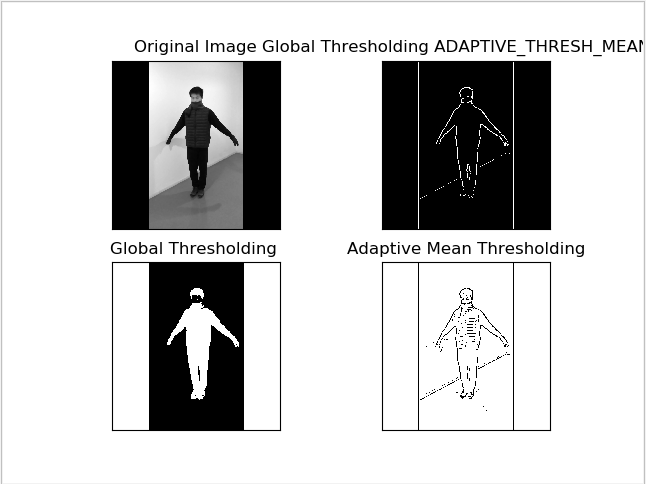
\includegraphics[width=12cm]{figure/mask_process}
	\caption{mask处理过程不同阶段示意图}
\end{figure}

\begin{figure}
	\centering
	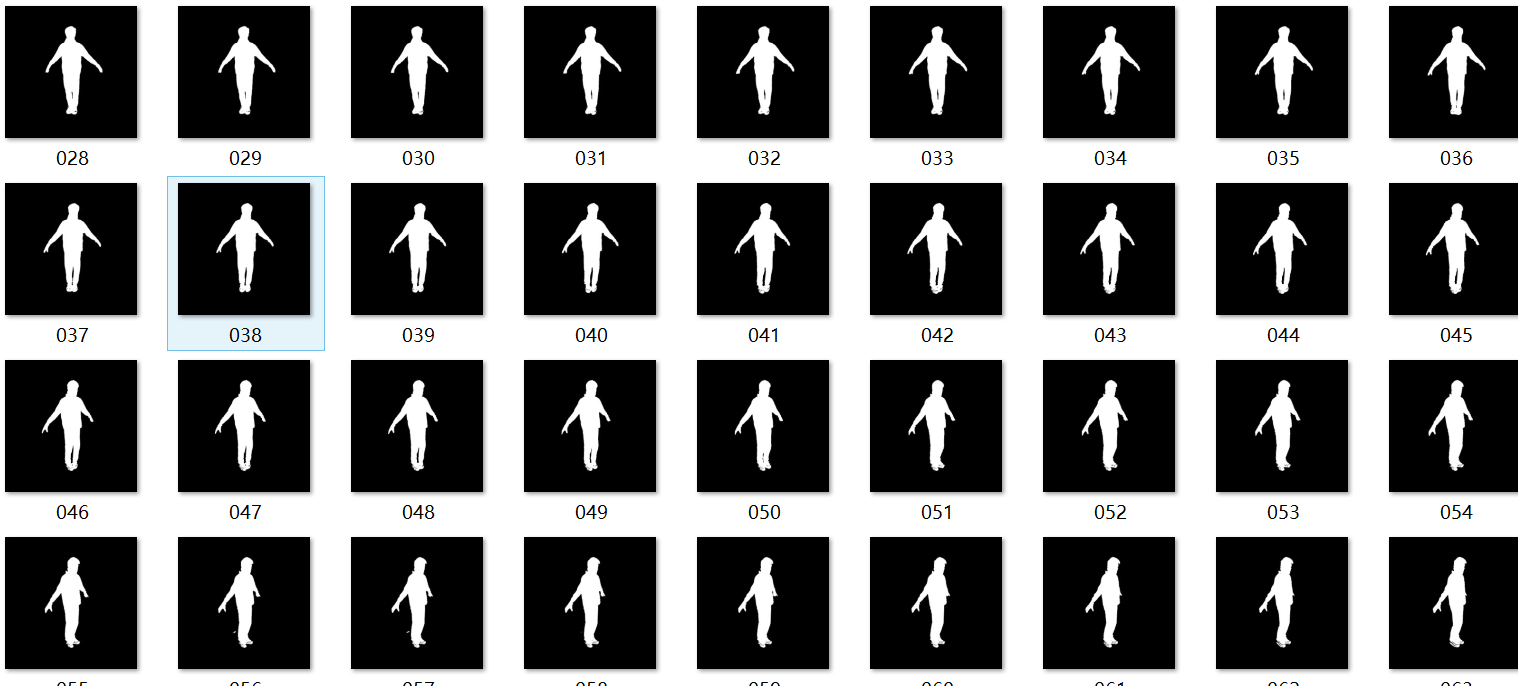
\includegraphics[width=16cm]{figure/mask_res}
	\caption{自拍视频抽取的关键帧的mask处理结果示意图}
\end{figure}

\subsubsection{人体关键点数据生成}
利用Openpose\cite{openpose}框架,我们得到了\cite{paper1,paper2}中需要的人躯体关键点数据和人的面部关键点数据。相关步骤不再赘述。

\begin{figure}
	\centering
	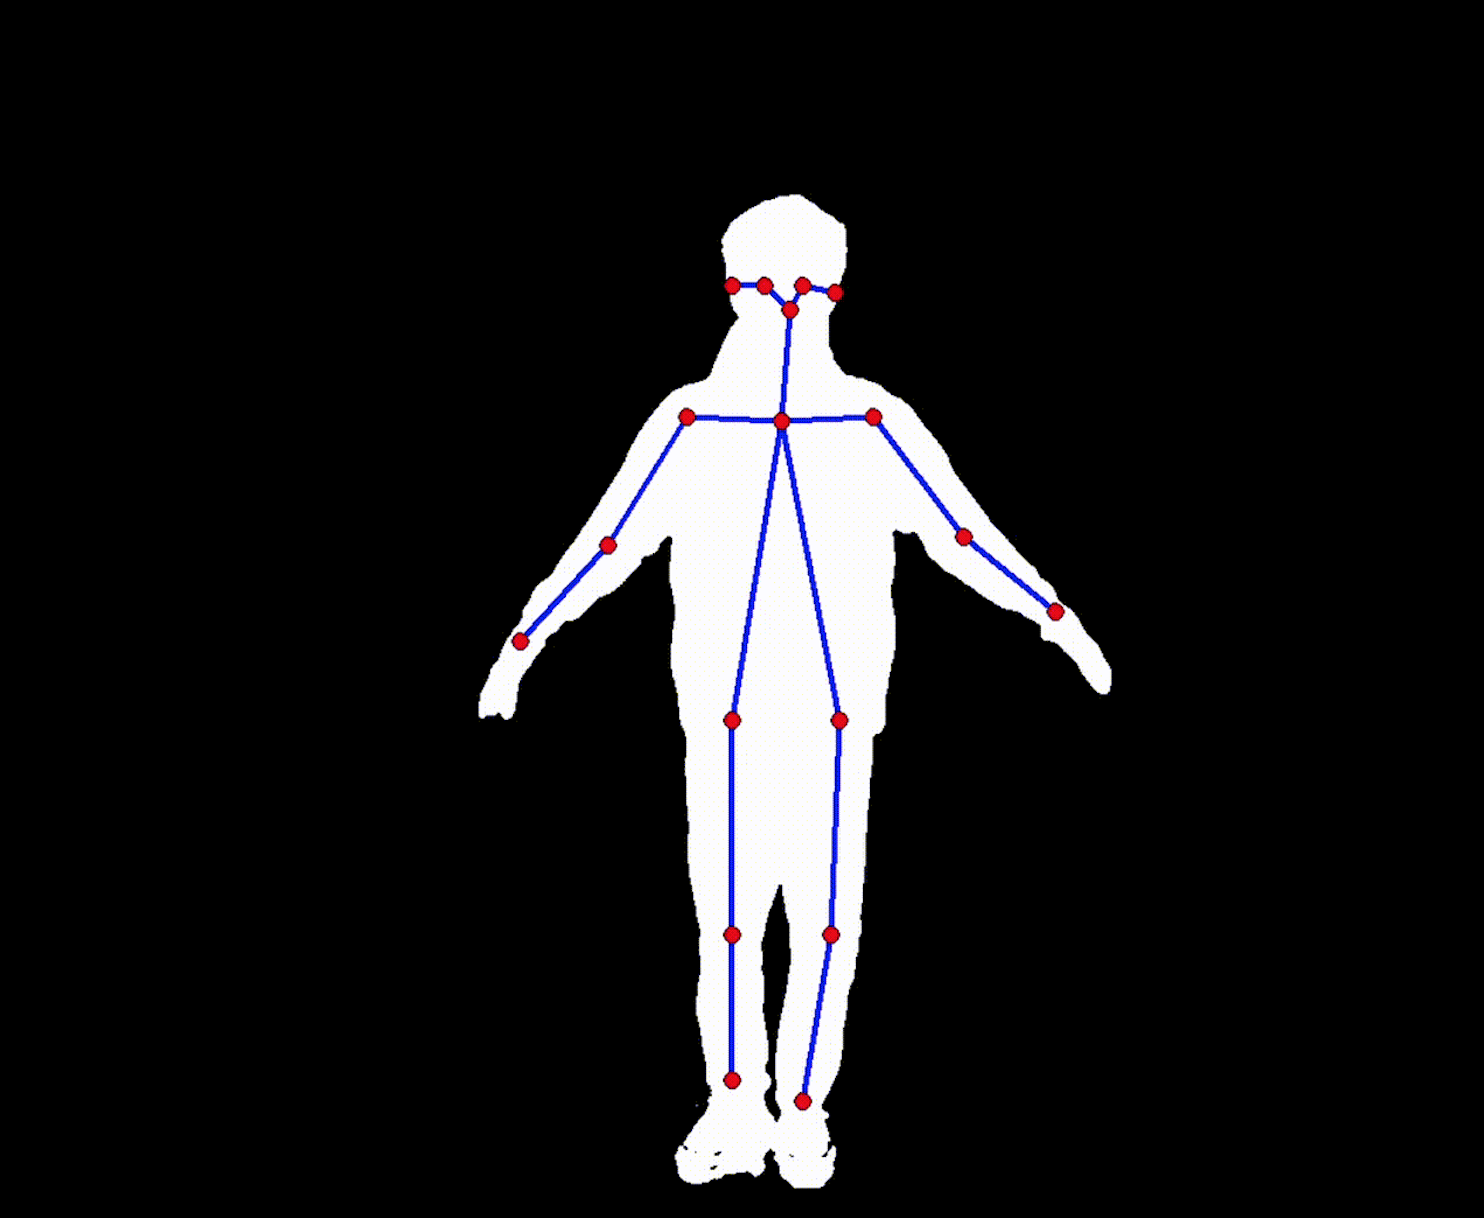
\includegraphics[width=12cm]{figure/kp_mask}
	\caption{综合了躯体关键点和mask信息的自拍视频抽样图}
\end{figure}

\subsection{实践过程}
在对自拍视频进行完数据的标定和预处理之后,便可以通过已经成功部署的videoavatar工程进行人体建模了,但是这个部分却让我们遇到了最多的困难,相关的细节可以参考Section 6.2。总而言之,我们最终得到了比较良好的自拍视频建模结果,Fig.\ref{huvideo}展示了部分的自拍视频关键帧截图,Fig.\ref{hures}展示了模型直接生成的人体建模结果和贴图。

\begin{figure}[H]
	\centering
	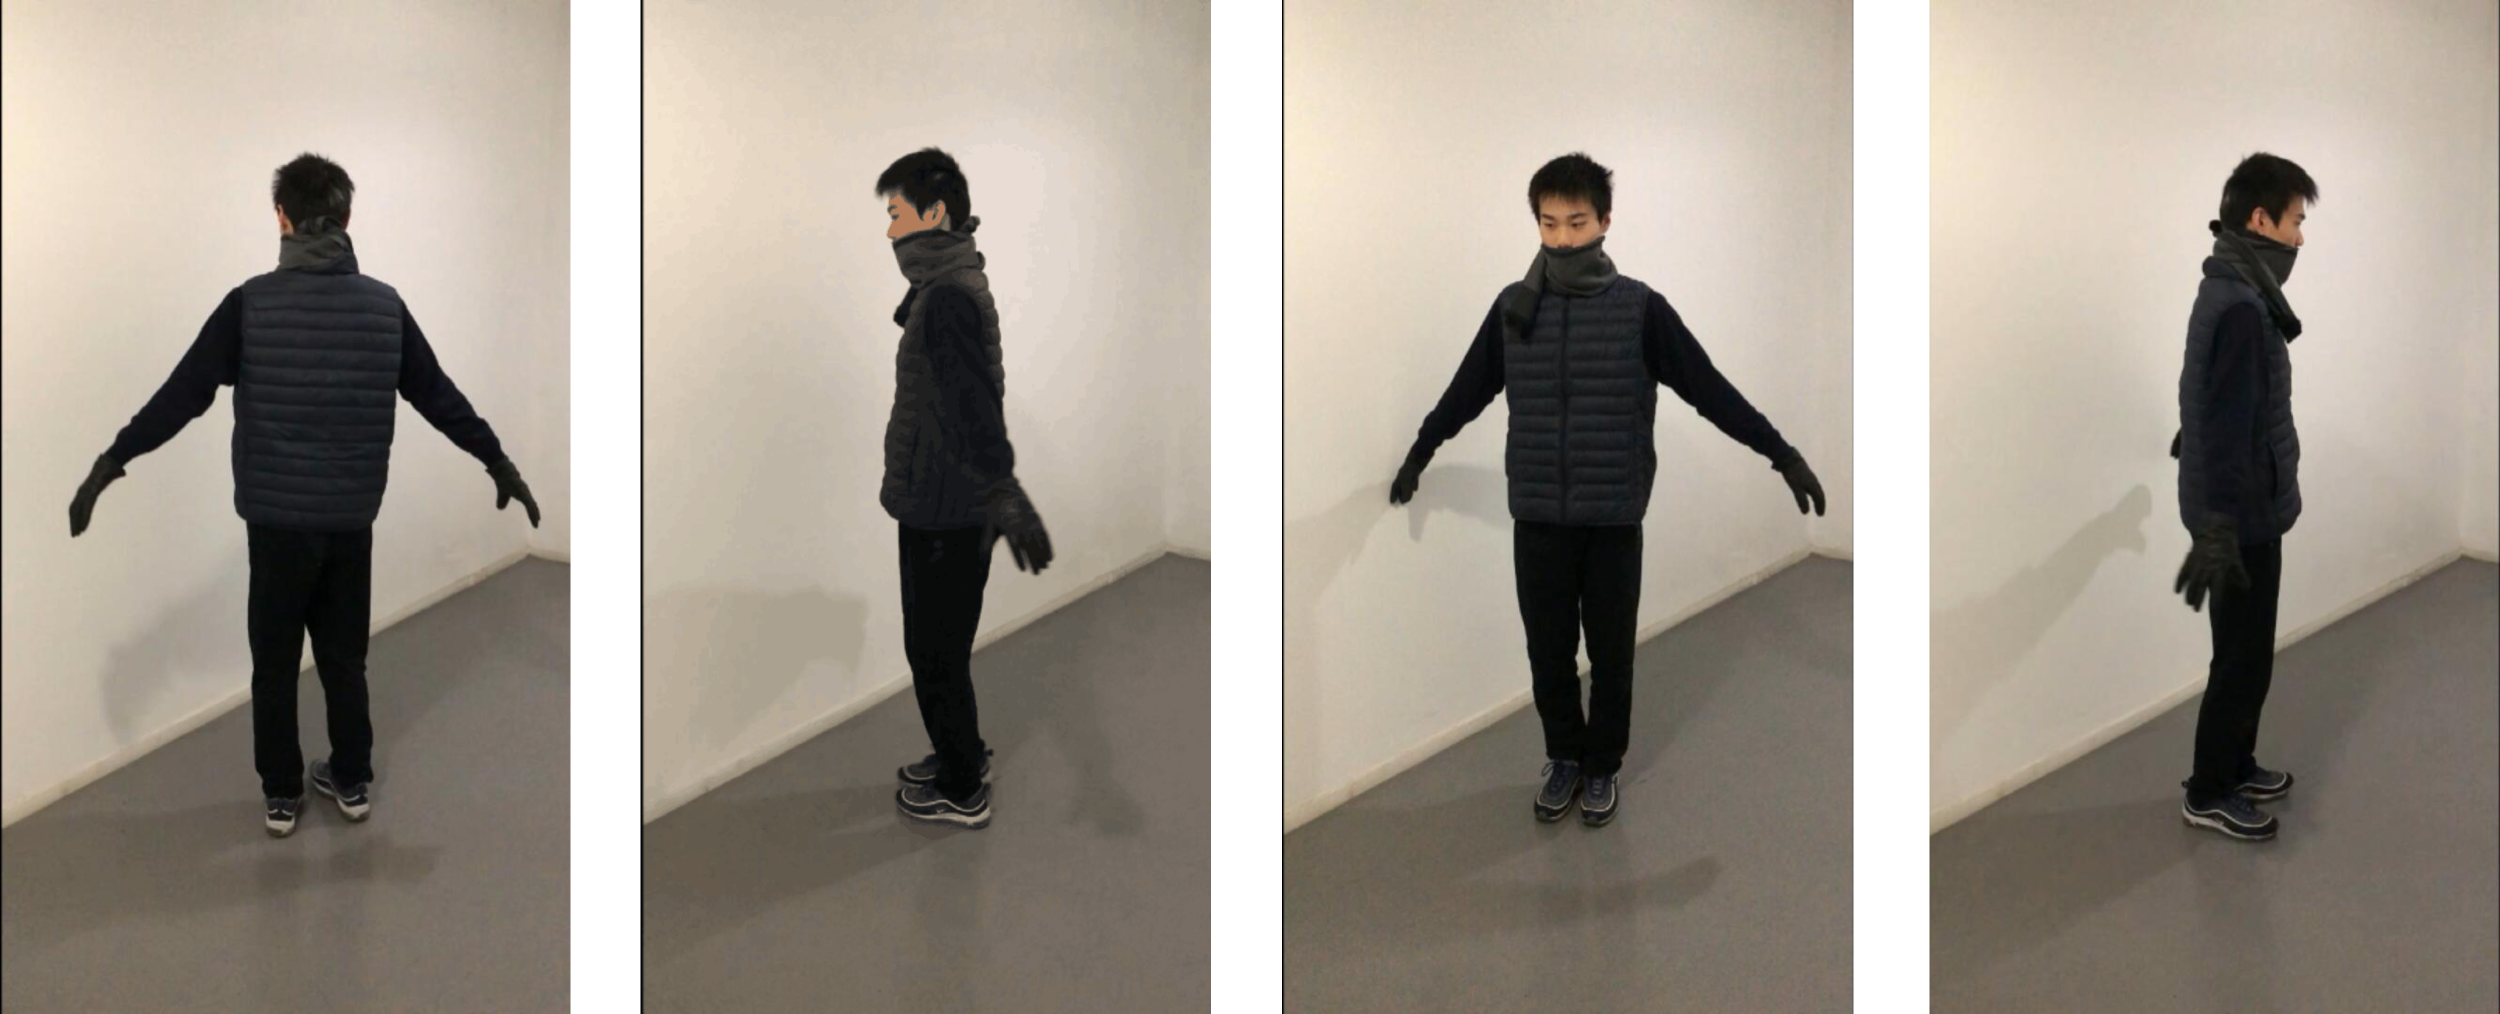
\includegraphics[width=14cm]{figure/huhuhu}
	\caption{从自拍视频中抽取的部分关键帧截图}
	\label{huvideo}
\end{figure}

\begin{figure}[H]
	\centering
	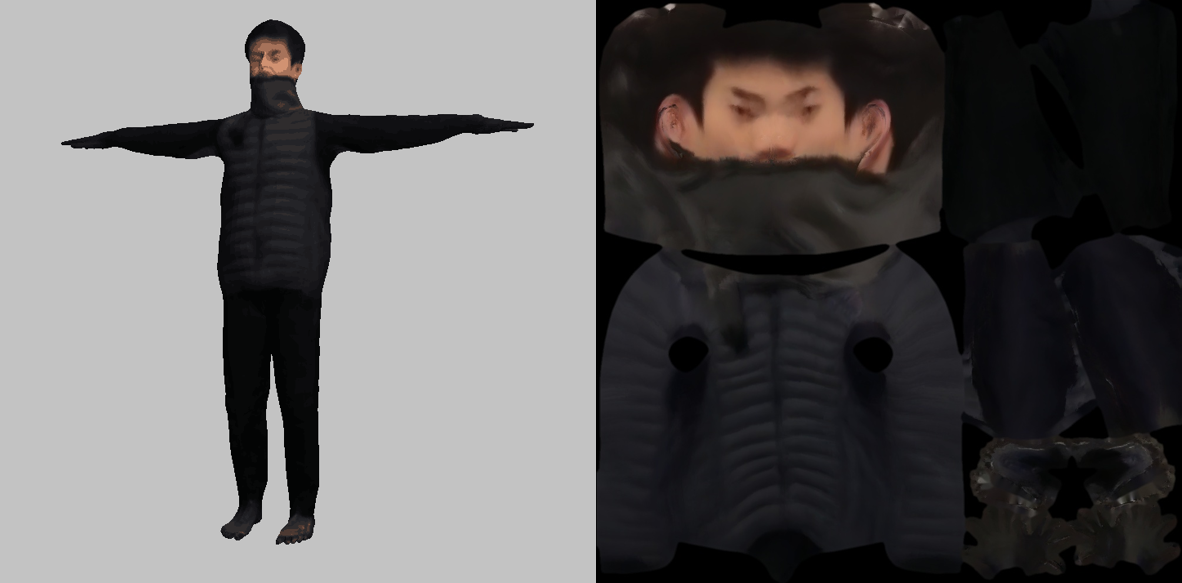
\includegraphics[width=14cm]{figure/selfshoot_res1}
	\caption{模型生成的自拍视频中的人物建模结果}
	\label{hures}
\end{figure}

此外,我们还利用了前述的面部细节优化方法,在自拍对象的面部采集了关键点,进行了面部细节的专门优化,效果展示在Fig.\ref{huface}。可以较为明显的看到,包括眼皮、眉骨、鼻翼等细节部分都进行了优化,得到了更加细致的效果。

\begin{figure}
	\centering
	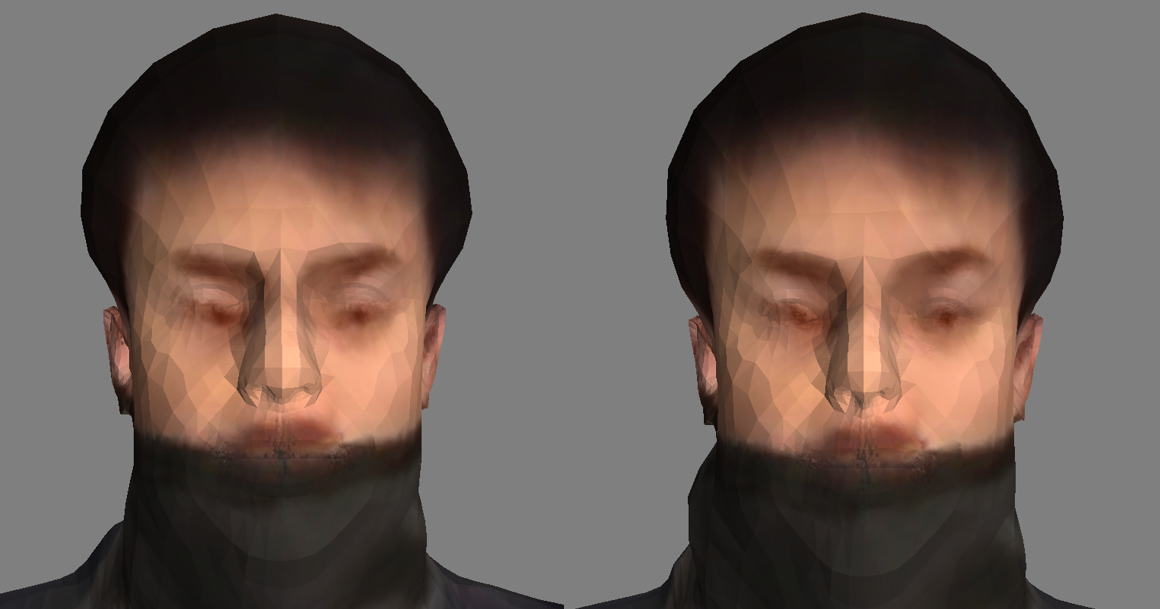
\includegraphics[width=14cm]{figure/selfshoot_Face_compare.png}
	\caption{对自拍目标进行面部细节优化的结果,左图为优化之前的效果,右图为优化之后的效果}
	\label{huface}
\end{figure}

\section{chumpy和opendr的代码移植}
SMPL的实现中使用了一个作者们自己包装的chumpy库,这个库只支持python2.x的版本,另一方面,video-avatar中还使用了opendr库进行相机标定等工作,opendr也只支持python2.x。因为这种兼容上的不足,给相关工作的复用带来了很多的不便,因此我们尝试将这两个关键的库文件进行移植,从而支持如今更加通用的python3.x。

\subsection{对python不兼容函数的复写}
python2.x和python3.x有诸多的底层函数互不兼容,主要有以下的几个部分:
\begin{itemize}
	\item 将python2.x中的print xxx复写为兼容python3.x的print(xxx)形式;
	\item reload函数不再作为内置函数,而被封装入imp;
	\item reduce函数不再作为内置函数,被封装入functools。
\end{itemize}

\subsection{import语法的修改}
python2与3的“absolute import”语法不同,即在同目录下的import .py文件的语法不同,如:
\begin{lstlisting}[language=python]
# 同目录下有utils.py
# import utils 			# python2
from . import utils 		# python3
    
# from t import * 			# python2
from .t import * 			# python3
\end{lstlisting}

\subsection{pickle库用法修改}
python2.x和python3.x的pickle库用法不同,需要进行修改。

\begin{lstlisting}[language=python]
# import cPickle as pkl 		# python2
import pickle as pkl 			# python3
	
# pkl.load(fp) 				# python2
pkl.load(fp,encoding='latin1')		# python3
\end{lstlisting}

\subsection{运算法"/"的修改}
python2中的除法是整除法,类似c语言,而python3中的单斜杠除法表示浮点除法,运算结果将被直接转换成浮点数,即使是整除,这会和numpy产生很多联合错误(矩阵的除法)。

\begin{lstlisting}[language=python]
# 将浮点型矩阵转换成整形矩阵(主要用于shape矩阵)
arr = arr.astype(np.int32) 	# shape矩阵必须是整型矩阵(会报错)
k = int(k)			# 将浮点数转换成整数

# 重载“/”符号 in ch.py
def __div__ (self, other):  		# python2 "/" ,需注释掉
	return ch_ops.divide(x1=self, x2=other)

def __truediv__ (self, other):  # python3 "/"
	return ch_ops.divide(x1=self, x2=other)
\end{lstlisting}

然而,如Fig.\ref{python2_div0}和Fig.\ref{python3_div0}中所示,在矩阵的运算中,当矩阵中存在零项的时候,可能会产生一些零除错,这个在numpy的实现中被特别处理了,但在我们的移植中仍可能发现一些小的问题,不过不影响opendr和chumpy工程文件的运行。

\begin{figure}[H]
	\centering
	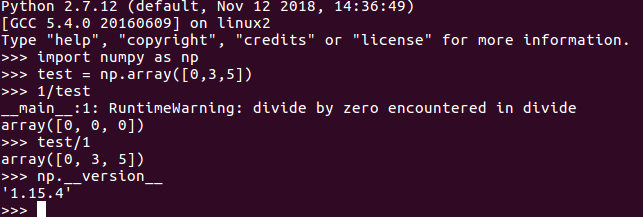
\includegraphics[width=14cm]{figure/python2_div0.png}
	\caption{零除错在python2版本中的体现:产生RuntimeWarning}
	\label{python2_div0}
\end{figure}

\begin{figure}[H]
	\centering
	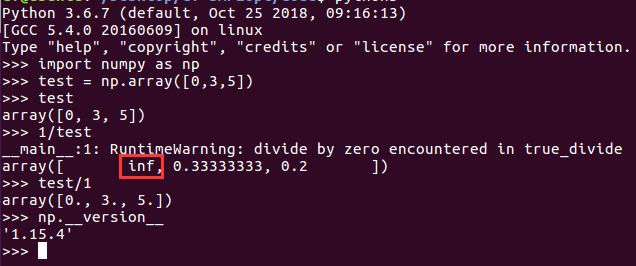
\includegraphics[width=14cm]{figure/python3_div0.png}
	\caption{零除错在python2版本中的体现:产生RuntimeWarning,对应项目变成inf字节}
	\label{python3_div0}
\end{figure}

\subsection{移植opendr的ctx\_mesa.so链接库}
opendr中使用了Cython编程,cython本质上是c和python语言的混合体,可以编译出让python直接import的动态链接库。ctx\_mesa.so主要是简化opengl的模块并完成opendr和opengl的对接。但是,python2与python3在Cython中的基础数据类型不一样,直接import python2的连接库会报数据结构找不到的错误。为了解决这个问题,需要做的是在python3环境下重新编译ctx\_mesa;并且在不同的环境下,比如移植到mac下,重新进行编译。在这个步骤中,我们假设并没有一个适配的ctx\_mesa文件,需要自己重新编译生成,具体的步骤为:

\begin{enumerate}
	\item 在进行重新编译之前,需要说明编译需要用到的素材文件,相关的素材文件列表见Appendix A;
	\item 修改 setup.py,使之满足python3语法,相关的要求见本节前半部分;
	\item 命令行执行安装指令:
	\begin{lstlisting} 
		$ python3 setup.py build_ext --inplace
	\end{lstlisting}
	\item 如果编译出ctx\_mesa开头的.so文件,则说明正确,修改文件名为ctx\_mesa.so替换即可,若出现额外报错,则修正后重新编译。
\end{enumerate}

\subsection{编译后与ctx\_mesa.so的OsContext类对接}
由于python2中str和bytes是同一个数据类型,可以直接传参对接,python3中需要先将str转换为bytes对象再传参,并且在在opendr库中的renderer.py中对接载入修改内容,最后opendr库中\_constants.py定义了一些与opengl对接的常数,需要在合适的位置进行import(都在原始代码的注释中,取消注释即可):
\begin{lstlisting}[language=python]
s = s.encode() # trans str to bytes
from opendr.contexts.ctx\_mesa import OsContext
from .contexts.\_constants import *
\end{lstlisting}

经过前述的步骤,得到的移植后的文件已经可以在Python3.x的环境下得到完整的运行。对于Opendr和chumpy有关代码的移植工作由此完成。
\section{总结}
\subsection{已完成的工作}
在本次的课程项目中,我们小组成员按照老师的要求,基于论文\cite{smpl}的基础模型和开源的\cite{paper1code}项目,进行了3D人体建模方面的探索学习。在大概一个月的团队工作之后,我们在若干方面取得了成果:

\begin{itemize}
	\item 对论文\cite{smpl,paper1,paper2}进行学习理解,定期提交进度报告,整理总结了论文的核心思想;
	\item 部署运行了videoavatar\cite{paper1code}项目工程,生成了动态的avatar效果;
	\item 自行拍摄视频,并对视频进行了较为成功的建模实验;
	\item 将已有的videoavatar项目移植到了Python3.x环境中,对其依赖的opendr和chumpy库进行了部分复写;
	\item 对论文\cite{paper1}的开源代码进行学习,进行参数调优,提高了模型的性能;
	\item 提取论文\cite{paper2}的算法思想,对包括Mesh细分、面部细节重建等关键步骤进行了实现,取得了效果;
	\item 制作了便捷的工具,使用videoavatar进行纹理贴图和渲染。
\end{itemize}
\subsection{失败的经验}
在本次课程项目的推进过程中,我们遭遇到了许多失败,我们相信失败的经验往往比成功的例子更加重要。
\subsubsection{对Shape-from-shading的复现失败}
论文\cite{paper2}在实现detailed video-avatar的时候,使用了一种精细的shape-from-shading\cite{shapefromshading}方法为模型优化提供重要的依据。但是该方法并的源代码并没有开源,我们尝试复现其论文的思想,但是因为该论文过多的前置知识依赖和含糊不清的参数说明,相关工作很快停滞,相关的复现尝试宣告失败。
\subsubsection{对自拍视频进行建模过程中的失败}
尽管我们小组最终较为理想地完成了对自拍视频的建模工作,但是付出了没有预料到的巨大时间代价,过程中遭遇到了诸多的困难乃至于失败。在最初的尝试中,我们得到了和自拍人物完全不相似的建模结果(如Fig.\ref{failure_1}),在尝试了几乎所有的参数调整后也没有任何的改善,只是得到了更多的形态各异的失败结果(如Fig.\ref{failure_2}),在对相机参数进行反复调节校准、对优化过程参数进行反复尝试失败之后,我们意外地发现失败的原因是在mask层面。如Fig.\ref{mask_mismatch}。在对视频进行关键帧的抽取之后,我们希望按照时间顺序把关键帧进行排序,如果每10帧抽取一个关键帧,我们希望前三个关键帧应当是第0、10、20帧,相邻关键帧之间应该有非常相近的人物姿态。但是如图所示,在对mask数据进行排序之后,第二个关键帧和第三个关键帧之间出现了明显的区别,经过错误排查发现是因为在数据“排序”的过程中,python内置的排序语句会得到:"0" < "1" < "10" < "100" < "2"的排序结果,这是因为对字符串匹配的逐位字符比对导致的。所以,我们的错误就是因为在建模中使用的关键帧序列是几乎完全乱序的,相邻帧之间的形态差异巨大,导致平滑的模型优化不可能被继续下去。

修正了这个错误之后,我们得到了预想的按照时间顺序排列的关键帧序列,抽样效果如Fig.\ref{frame_order}所示。

\begin{figure}
	\centering
	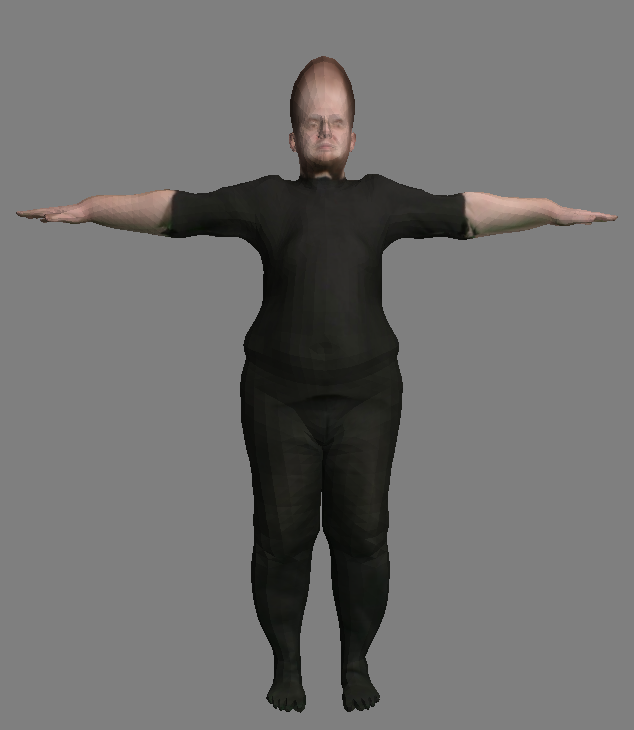
\includegraphics[width=5cm]{figure/failure_1.png}
	\caption{最初的自拍人物建模失败样例}
	\label{failure_1}
\end{figure}

\begin{figure}
	\centering
	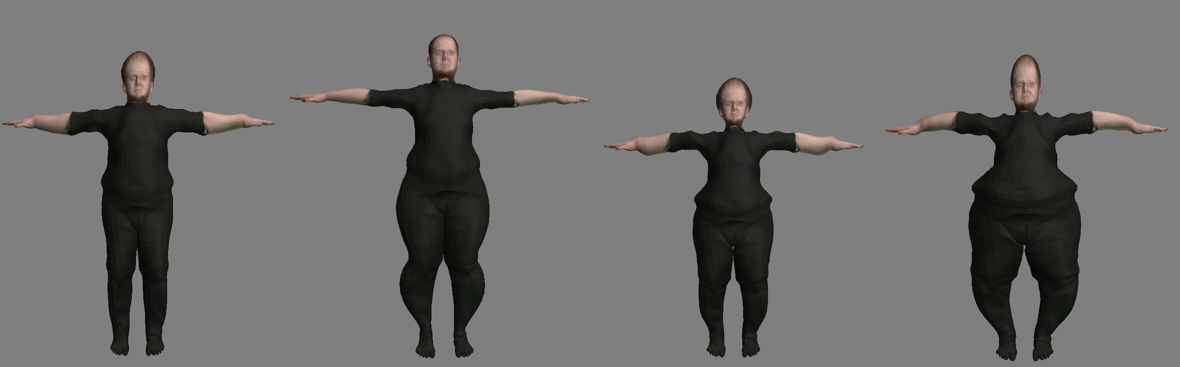
\includegraphics[width=14cm]{figure/failure_2.png}
	\caption{尝试各种参数调整之后仍旧失败,得到了形态各异单就是不像视频人物的建模结果}
	\label{failure_2}
\end{figure}


\begin{figure}
	\centering
	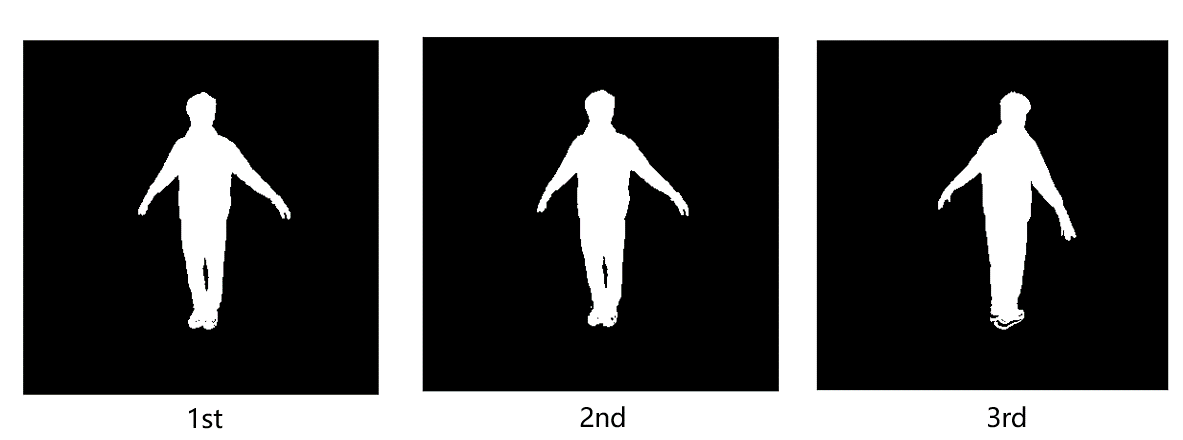
\includegraphics[width=15cm]{figure/frame_mismatch.png}
	\caption{在对原始的mask图片进行“排序”之后得到的前三个关键帧剪影效果}
	\label{mask_mismatch}
\end{figure}

\begin{figure}
	\centering
	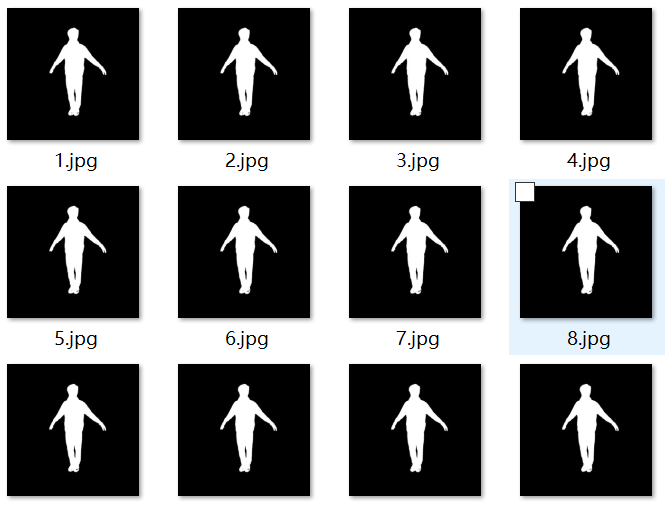
\includegraphics[width=14cm]{figure/frame_wrong_order.png}
	\caption{在进行重新排序后得到的关键帧序列}
	\label{frame_order}
\end{figure}

\subsection{进一步工作}
因为时间和精力的限制,我们仍有诸多的技术目标没有达成,包括:

\begin{itemize}
	\item 完整实现论文\cite{paper2}中的技术方案,包括shape-from-shading-based的细节优化和纹理优化等;
	\item 实现模型的并行化计算,解决当前项目文件效率过低的问题;
	\item 将chumpy库解开,移植到numpy等兼容性更好、效率更高、支持GPU运算和高级内存优化的库依赖环境下。
\end{itemize}

\newpage
\bibliographystyle{abbrv}
\bibliography{ref}

\clearpage

\begin{appendices}
\section{编译ctx\_mesa.so需要的素材文件}
\begin{lstlisting} 
cv@ubuntu:~/Desktop/opendr/contexts$ tree -L 4
.
|-- autogen.py
|-- _constants.py
|-- ctx_base.pyx
|-- ctx_mac_internal.c
|-- ctx_mac_internal.h
|-- ctx_mac.pyx
|-- ctx_mesa.c
|-- ctx_mesa.pyx
|-- ctx_mesa.so(这个是最后的输出)
|-- draw_triangle_shaders_2_1.py
|-- draw_triangle_shaders_3_2.py
|-- fix_warnings.py
|-- _functions.pyx
|-- gl_includes.h
|-- __init__.py
|-- Makefile
|-- OSMesa
|   |-- include
|   |   |-- GL
|   |       |-- glext.h,gl.h,gl_mangle.h,glu.h,glu_mangle.h,glxext.h
|   |       |-- glx.h,glx_mangle.h,osmesa.h,vms_x_fix.h,wglext.h,wmesa.h
|   |-- lib
|       |-- libGL.a
|       |-- libGLU.a
|       |-- libOSMesa.a
|       |-- pkgconfig
|           |-- gl.pc
|           |-- glu.pc
|           |-- osmesa.pc
|-- __pycache__

6 directories, 34 files
\end{lstlisting}

\section{Subdivision中建立smpl模型图矩阵}
\begin{lstlisting}[language=python]
def add_new_node():
    ii = 0
    for x in f:
        ii= ii+1
        global node_num,row,col,data,new_node_position,v_template
        x0 = x[0]
        x1 = x[1]
        x2 = x[2]
        s01 = str(x0)+str(x1)
        s10 = str(x1)+str(x0)
        s02 = str(x0)+str(x2)
        s20 = str(x2)+str(x0)
        s12 = str(x1)+str(x2)
        s21 = str(x2)+str(x1)
        v0 = 0
        v2 = 0
        v1 = 0
        if dict.has_key(s01) == False:
            dict[s01] = node_num
            dict[s10] = node_num
            v0 = node_num
            new_node_position[node_num-6890][0] = \\
            	(v_template[x0][0] +v_template[x1][0])/2
            new_node_position[node_num-6890][1] = \\
            	(v_template[x0][1] +v_template[x1][1])/2
            new_node_position[node_num-6890][2] = \\
            	(v_template[x0][2] +v_template[x1][2])/2
            node_num = node_num+1
            row = np.concatenate([row,[x0,v0,x1,v0]])
            col = np.concatenate([col,[v0,x0,v0,x1]])
            data = np.concatenate([data,[1,1,1,1]])
        else:
            v0 = dict[s01]
        if dict.has_key(s02) == False:
            dict[s02] = node_num
            dict[s20] = node_num
            v1 = node_num
            new_node_position[node_num-6890][0] = \\
            	(v_template[x0][0] +v_template[x2][0])/2
            new_node_position[node_num-6890][1] = \\
            	(v_template[x0][1] +v_template[x2][1])/2
            new_node_position[node_num-6890][2] = \\
            	(v_template[x0][2] +v_template[x2][2])/2
            node_num = node_num+1
            row = np.concatenate([row,[x0,v1,x2,v1]])
            col = np.concatenate([col,[v1,x0,v1,x2]])
            data = np.concatenate([data,[1,1,1,1]])
        else:
            v1 = dict[s02]
        if dict.has_key(s12) == False:
            dict[s12] = node_num
            dict[s21] = node_num
            v2 = node_num
            new_node_position[node_num-6890][0] = \\
            	(v_template[x1][0] +v_template[x2][0])/2
            new_node_position[node_num-6890][1] = \\
            	(v_template[x1][1] +v_template[x2][1])/2
            new_node_position[node_num-6890][2] = \\
            	(v_template[x1][2] +v_template[x2][2])/2
            node_num = node_num+1
            row = np.concatenate([row,[x1,v2,x2,v2]])
            col = np.concatenate([col,[v2,x1,v2,x2]])
            data = np.concatenate([data,[1,1,1,1]])
        else:
            v2 = dict[s12]
        row = np.concatenate([row,[v0,v1,v0,v2,v1,v2]])
        col = np.concatenate([col,[v1,v0,v2,v0,v2,v1]])
        data = np.concatenate([data,[1,1,1,1,1,1]])	
        
# 生成稀疏矩阵:
adj = sp.coo_matrix((data,(row,col)),shape=(node_num,node_num))	
\end{lstlisting}

由于考虑到了内存不够的问题,我们这里使用了稀疏矩阵。因为该矩阵中大多数位置都为0,每个点之和其周围的6个点相连。我们只要记录矩阵中有数据的row和col,即可还原出整个矩阵。

\section{自制obj文件可视化工具}
我们小组针对生成videoavatar中需要进行的渲染和可视化工作开发了一个简易的一键操作工具\cite{renderingtool},对其用法进行简要的介绍:

\subsection{方法1:通过.bat文件运行}
如图Fig.\ref{renderrun},将含有模型和贴图的文件夹拖到 run.bat 上运行即可,这种方法较为简便,是推荐方案。
\begin{figure}
	\centering
	
\includegraphics[width=16cm]{figure/rendertool_run}
	\caption{使用批处理文件可以一步运行该工具}
	\label{renderrun}
\end{figure}

\subsection{方法2:通过loader.exe文件运行}
命令行运行:
\begin{lstlisting}
> loader.exe 

// 在弹窗中输入模型文件即可:
(cout) Model path:
(cin)  path_to_model_file
\end{lstlisting}

Fig.\ref{rendering1}给出了利用该渲染工具得到的效果示意图。
\begin{figure}
	\centering
	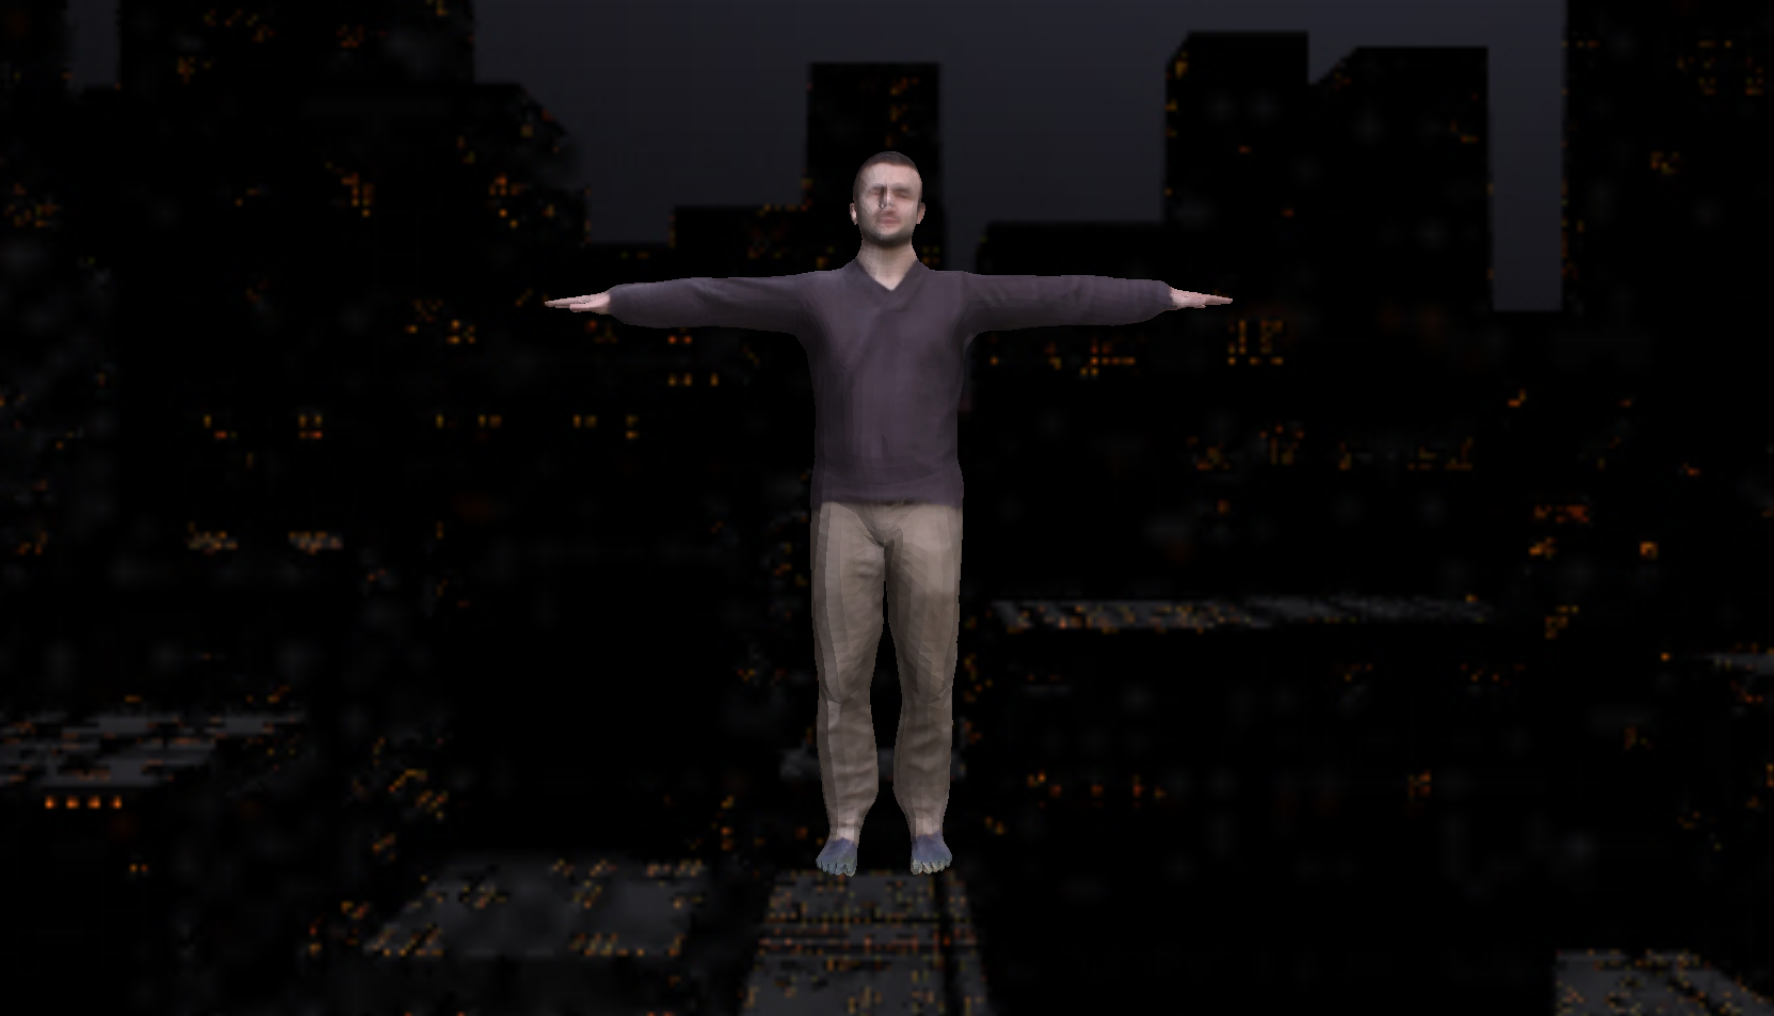
\includegraphics[width=14cm]{figure/rendering1}
	\caption{利用渲染工具生成的渲染效果图}
	\label{rendering1}
\end{figure}

\section{面部细节优化的工程复现}
\begin{lstlisting}[language=python, title=face2hdf5.py]
with h5py.File(out_file, 'w') as f:
    poses_dset = f.create_dataset("face_landmark", (len(pose_files), 70*3), 'f', chunks=True, compression="lzf")
    
    for i, pose_file in enumerate(tqdm(pose_files)):
        with open(pose_file) as fp:
            pose = np.array(json.load(fp)['people'][0]['face_keypoints'])
            poses_dset[i] = pose
\end{lstlisting}
\begin{lstlisting}[language=python, title=bodypart.py]
def get_face_vertex_ids():
        v_ids = get_bodypart_vertex_ids()
        return v_ids['face']
\end{lstlisting}  
\begin{lstlisting}[language=python, title=frame.py]
def setup_frame_rays(base_smpl, camera, camera_t, camera_rt, pose, trans, mask)
def setup_frame_rays_paper2(base_smpl, camera, camera_t, camera_rt, pose, trans, mask, face_landmark)
# 新函数比原来多了一个face_landmark参数,指的是这一帧的面部landmark数据
def setup_frame_rays_paper2(base_smpl, camera, camera_t, camera_rt, pose, trans, mask, face_landmark):
        ... //与原函数相同
        
        # paper2
    
        # shape (70,3)->(x,y,scores)
        f.face_landmark = np.array(face_landmark).reshape(-1, 3) 
        f.face_rays = rays_from_landmark(f.face_landmark, camera)
    
        return f

# 为每一个frame对象新增了face_landmark和face_rays两个属性
# face_landmark:对应70个面部关键点的(x, y, confidence_score),shape为(70,3)
# face_rays:由face_landmark得到的2D投影光线,shape为(70, 2, 3)
\end{lstlisting}  
\begin{lstlisting}[language=python, title=rays.py]
def rays_from_landmark(landmark, camera):
        points = landmark[:,:-1] #array((x1,y1)(x2,y2)...)
        rays = rays_from_points(points, camera)
        return rays
        
def select_rays函数中还返回了一个w—_idx,z这一项对应论文中:
    (rays, Vi, smpl, face_ids):
        # find face vertexs 
        v_ids = face_ids
        verts = smpl.r[v_ids]
    
        # calculate vert-ray distance
        n, m = plucker(rays)
        dist = np.linalg.norm(np.cross(verts.reshape(-1, 1, 3), n, axisa=2, axisb=1) - m, axis=2)

        # for every ray, find closest vertex
        ray_matches = np.argmin(dist, axis=0) #for each ray -> idx of closest vertex
        vert_matches = np.argmin(dist, axis=1) #for each vertex -> idx of closest ray
        
        # unpose rays
        ...
        
        # find valid matching
        valid_rays = dist[np.vstack((ray_matches, range(dist.shape[1]))).tolist()] < 0.12
        valid_verts = dist[np.vstack((range(dist.shape[0]), vert_matches)).tolist()] < 0.03
         
        ray_matches = ray_matches[valid_rays]
        
        # idx of w - w: confidence of landmark
        w_idx = np.concatenate((np.arange(rays.shape[0])[valid_rays], vert_matches[valid_verts]))
         
        return np.concatenate((v_ids[ray_matches], v_ids[valid_verts])), \
               np.concatenate((rays_u_r[valid_rays], rays_u_v[valid_verts])),\
               w_idx
               
def ray_face(f, sigma, base_smpl, camera, face_ids):
        camera.t[:] = f.trans  
        ...
\end{lstlisting}  
\begin{lstlisting}[title=step2\_consencus.py, language=python]  
# part 1: main函数中增加参数face_file, 进行预处理
def main(pose_file, masks_file, face_file, camera_file, ...):

	# load face_landmarks.h5
    # @face_file : file name of face landmarks face_landmarks.hdf5
    face_data = h5py.File(face_file, 'r')
    face_landmark = face_data["face_landmark"][first_frame:last_frame]
    
    # init
        ...
    
    for i in indices_consensus:
       	log.info('Set up frame {}...'.format(i))
		mask = ...
        pose_i =. ..
        trans_i =...

# 得到这一帧的landmark数据,进行setup
	face_i = np.array(face_landmark[i], dtype=np.float32)
	frames.append(setup_frame_rays_paper2(base_smpl, camera, camera_t, camera_rt, pose_i, trans_i, mask, face_i))

# 调用fit_consensus进行模型优化
	log.info('Set up complete.')
	log.info('Begin consensus fit...')
	fit_consensus(frames, base_smpl, camera, frustum, model_data, nohands, icp_count, naked, display)
        
	...	# save data

# part 2: 在fit_consensus中加入E_{face}能量项,参与模型优化
face_ids = get_face_vertex_ids() # 获取面部的vertex
     
# 其他能量项
E = {
  'laplace': (sp_dot(L, base_smpl.v_shaped_personal) - delta) * w_laplace,
  'model': (base_smpl.v_shaped_personal - model_template) * w_model,
  'symmetry': (base_smpl.v_personal + np.array([1, -1, -1])* base_smpl.v_personal[model_data['vert_sym_idxs']]) * w_symmetry,
}

# 为每一帧增加能量项E_{face}
log.info('## Matching rays with contours')
for current, f in enumerate(tqdm(frames)):
	E['silh_{}'.format(current)] = ray_objective(f, sigma, base_smpl, camera, vis_rn_b, vis_rn_m)            

	E['face_{}'.format(current)] = ray_face(f, sigma, base_smpl, camera, face_ids) 

\end{lstlisting}

\end{appendices}

\end{document}
